\documentclass[draftspec]{sbmlpkgspec}
\usepackage{microtype}

\newcommand{\fixttspace}{\hspace*{1pt}}

\newcommand{\sbmlthreedynamic}{SBML Level~3 Package Specification for Dynamic Structures, Version~1\xspace}
\newcommand{\sbmlthreecore}{SBML Level~3 Version~2 Core\xspace}

%To remove when validationrules.tex is modified
\newcommand{\Dimension}{\defRef{Dimension}{sec:dimension}\xspace}
\newcommand{\ListOfDimensions}{\defRef{ListOfDimensions}{sec:dimension}\xspace}
\newcommand{\Index}{\defRef{Index}{sec:index}\xspace}
\newcommand{\ListOfIndices}{\defRef{ListOfIndices}{sec:index}\xspace}

\newcommand{\SpatialComponent}{\defRef{SpatialComponent}{subsec:spatialComp}\xspace}
\newcommand{\ListOfSpatialComponents}{\defRef{ListOfSpatialComponents}{subsec:listSpatialComp}\xspace}
\newcommand{\Behavior}{\absDefRef{Behavior}{Behavior-class}}
\newcommand{\Behaviors}{\absDefRef{Behaviors}{Behavior-class}}

\newcommand{\Element}{\defRef{Element}{subsec:Element}\xspace}
\newcommand{\ListOfElements}{\defRef{ListOfElements}{subsec:ListOfElements}\xspace}

\newcommand{\ListofGroups}{\textbf{\class{ListofGroups}}\xspace}


\newcommand{\Compartments}{\textbf{\class{Compartments}}\xspace}
\newcommand{\Reactions}{\textbf{\class{Reactions}}\xspace}
\newcommand{\Parameters}{\textbf{\class{Parameters}}\xspace}
\newcommand{\ChangedMath}{\textbf{\class{ChangedMath}}\xspace}


\begin{document}

\packageTitle{Qualitative Models}
\packageVersion{Version 1.0 (Draft)}
\packageVersionDate{22nd Aug 2012}
\packageGeneralURL{http://sbml.org/Documents/Specifications/SBML_Level_3/Packages/Qualitative_Models_(qual)}
\packageThisVersionURL{}

\author{%
  \begin{tabular}{c>{\hspace{20pt}}c}
    Claudine Chaouiya			          & Sarah M Keating\\[0.25em]
    \mailto{chaouiya@igc.gulbenkian.pt}	  & \mailto{skeating@ebi.ac.uk}\\[0.25em]
    IGC Rua da Quinta Grande 6                 & European Bioinformatics Institute\\
    P-2780-156 Oeiras                              & Cambridgeshire\\
    Portugal	                                         & UK\\
\\
\\
    Duncan Berenguier			          & Aurelien Naldi\\[0.25em]
    TAGC INSERM U928                              &Center for Integrative Genomics\\
    13288 Marseille                                    & CH-1015 Lausanne\\
    France	                                                 & Switzerland\\
\\
\\
    Denis Thieffry      			          & Martijn P. van Iersel\\[0.25em]
    IBENS                                                    & European Bioinformatics Institute\\
    75005 Paris                                          & Cambridgeshire\\
    France  	                                         & UK\\
  \end{tabular}
}

\frontNotice{This is a working draft of the specification for the SBML Level 3
  package ``\texttt{qual}''.  It is not a normative document.  Please send
  comments and other feedback to the Package Working Group mailing list,
  \mailto{sbml-qual@lists.sourceforge.net}.}

\maketitlepage
\maketableofcontents

% -*- TeX-master: "multi" -*-

%%%%%%%%%%%%%%
% introduction
%%%%%%%%%%%%%%
\section{Introduction}
\label{def:Introduction}

This Multistate, Multicomponent and Multicompartment Species (Multi) package provides an extension of \SbmlLevelThreeWC\ that supports encoding \smodels\ with molecular complexes that have multiple components and can exist in multiple states and in multiple \compartments. One of its \mBlockChangedBegin{\revTwentyTwentyMarch}goals is\mBlockChangedEnd{\revTwentyTwentyMarch} to provide a platform for sharing \smodels\ based on the specifications of \mBlockChangedBegin{\revTwentyTwentyMarch} molecular transformations/interactions and the rules governing such reactions\mBlockChangedEnd{\revTwentyTwentyMarch} [\cite{ref:simmune2012, ref:scienceSignaling2006, ref:FeretPnas2009, ref:modeler2013}]. This specification covers the goals and features described in \multiOneProposalWC\ for extending SBML to carry the information for \textit{multistate multicomponent} \species\ with revised data structure. In addition, this specification includes the feature for \textit{multicompartment} \species\ as described in the releases of the Multi proposal [\cite{ref:multiproposal280}, \cite{ref:revisedMulti}].

\subsection{Proposal and specifications}
\label{def:Proposal}

The proposal corresponding to this package specification is available at:

\hspace{3ex}\url{http://sbml.org/Community/Wiki/SBML_Level_3_Proposals/Multistate_and_Multicomponent_Species_Proposal}

The specifications (v1.0.1 to current) are located at: 

\hspace{3ex}\url{https://sourceforge.net/p/sbml/code/HEAD/tree/trunk/specifications/sbml-level-3/version-1/multi/spec/}

\subsection{Package dependencies}
\label{def:Package_dependencies}

The Multi package has no dependencies on other \SbmlLevelThree\ packages.

\subsection{Document conventions}
\label{def:Document_conventions}

UML 1.0 notation is used in this document to define the constructs provided by this package. Colors 
in the diagrams carry the following additional information for the benefit of those viewing the 
document on media that can display color:

\begin{itemize}
 \item {\color{black}\framebox{\textit{Black}}} Items colored black are components taken unchanged 
      from their definitions in the \SbmlLevelThreeCore\ specification document.
 \item {\color{mediumgreen}\dbox{\textit{Green}}} Items colored green are components that exist in 
      \SbmlLevelThreeCore, but are extended by this package. Class boxes are also drawn with with 
      dashed lines to further distinguish them.
 \item {\color{sbmlblue}\framebox{Blue}} Items colored blue are new components introduced in this 
      package specification. They have no equivalent in  the \SbmlLevelThreeCore\ specification. 
\end{itemize}
 
For other matters involving the use of UML, XML and typographical conventions, this document follows the conventions
used in the \SbmlLevelThreeCore\ specification document [\cite{ref:sbmll3v1}].

For simplicity, \val{...} in all example code refers to some unspecified code content, that is not important for the purpose of illustrating the issue at hand.

% -*- TeX-master: "multi" -*-

\section{Background and context}
\label{def:Background}

Rule-base, domain-detailed modeling has been extremely valuable in systems biology related studies [\cite{ref:nathan2015} and \cite{ref:jamesFader2013}]. Rule-based, domain-detailed modeling approaches (\BioNetGen\ [\cite{ref:bionetgen2009}], \Kappa\ [\cite{ref:kappa2004}], and \Simmune\ [\cite{ref:simmune2012, ref:simmune2006}]) define rules for interactions between pairs of molecule domains, specifying how the interactions depend on particular states of the molecules (pattern) and their locations in specific compartments. In order to generate networks of biochemical reactions these rules are applied to the molecular components of the systems to be modeled, either at the beginning of the modeling (simulation) process or ``on the fly'' (as molecule complexes emerge from the interaction rules). Expressing such rule-based, domain-detailed reaction networks using the concepts of \Species and \Compartment in SBML (L3 core and L2) can be difficult for rules and molecule sets that lead to large numbers of resulting molecular complexes. It would therefore be desirable to have an SBML standard for encoding rule-based, domain-detailed \smodels\ using their ``native'' concepts for describing reactions instead of having to apply the rules and unfold the networks prior to encoding in an SBML format.

We proposed a revised proposal of the \multi\ package: ``Multistate, Multicomponent and Multicompartment Species Package for SBML Level 3''  (abbreviated as Multi) [\cite{ref:revisedMulti} and \cite{ref:multiproposal280}] which takes the scopes and some data structures developed in \multiOneProposalWC\ and addresses main issues arising from a rule-based, domain-detailed modeling point of view with the data structures consistent with that used in the available rule-based, domain-detailed modeling tools. 

\label{def:OtherRuleBasedModels}
\noticeFont{Note: \\
This specification was developed with the main goal of taking into account bi-molecular interactions mediated through specific binding domains (or sites). Models without such detailed description of the molecular interactions can be encoded as well if the other features in this specification such as \SpeciesFeatureType, \SpeciesFeature, and extended \ExCompartment satisfy the model requirements.
}


%-------------------------------------------------------
\subsection{Past work on this problem or similar topics}
\label{def:Past_work}

\begin{itemize}
 \item 
  Nicolas Le Nov\`ere and Anika Oellrich proposed the previous version of the Multi proposal [\cite{ref:multi1}]. However, it was realized that a more detailed treatment of molecular binding sites and their state-dependent interactions would be desirable.
 
 \item In August 2012, Fengkai Zhang from the \Simmune\ group presented `` Draft for discussion SBML Proposals for Revised Multi, Simple Spatial and Multi-Spatial Extensions'' at COMBINE 2012 [\cite{ref:revisedMulti}]. The three proposals cover the goals and scope of \multiOneProposal, revise it and add some new features that improve usage of the proposal for rule-based approaches.
 
 \item Based on the discussions and suggestions received during COMBINE 2012 as well as on feedback from the SBML discussion forum, \multiTwoProposalVerTwo\ was released to the SBML-Multi community, which integrates and covers most of the features in the three previous proposals of August 2012. 
 
 \item In May 2013, a new revision (rev 280) of the Multi proposal [\cite{ref:multiproposal280}] was released before the meeting of HARMONY 2013. The extended \ExCompartment class and its related classes have been reorganized. All optional boolean attributes have been removed/replaced. A new optional Multi attribute, \val{whichValue}, was added to the \token{ci} elements in \class{KineticLaw} to identify  the sources of \species. (Lucian Smith gave many comments/suggestions about this proposal and William Hlavacek gave thoughtful feedback about the \BioNetGen\ example in this proposal). This revision (rev 280) was presented at HARMONY 2013  [\cite{ref:harmony2013}] with new features to configure multiple occurrences of \SpeciesFeatureType. Several new or revised features were discussed during and after HARMONY 2013, including multiple occurrences of \SpeciesFeatureType, multiple copies of \SpeciesTypeInstance, the \numericValueAtt\ attribute for \PossibleSpeciesFeatureValue and concentration summation of pattern \species. These features are covered or updated in the specifications from v1.0.1.
  
\end{itemize}

%-------------------------------------------------------
\subsection{Revision history}
\label{def:revision_history}

The versioning convention used in this document: \\
\objFont{x.y.z (status)}

\objFont{x}: version of SBML Level 3 core. \\
\objFont{y}: version of the Multi package. \\
\objFont{z}: release of the Multi package at its version \objFont{y}. \\ 
\objFont{status}: \val{draft}, \val{release candidate}, or \val{release}. 

For example, the current version is \val{1.1.rc4 (release candidate)} \\
\objFont{x} = \val{1} \\
\objFont{y} = \val{1} \\
\objFont{z} = \val{rc4} \\
\objFont{status} = \val{release candidate} \\

The followings are the revision history of the Multi package:

\subsubsection{Version: 1.1.rc4 (release candidate), this version}
\label{def:v1_1_rc4}

More updates on validation rule numbers, line breaks, and the example about \SubListOfSpeciesFeatures. 

\subsubsection{Version: 1.1.rc3 (release candidate), Febrary 2017}
\label{def:v1_1_rc3}

Modify the numbers of several rules to be consistent with the general SBML validation rule conventions. 

\subsubsection{Version: 1.1.rc2 (release candidate), January 2017}
\label{def:v1_1_rc2}

Add a new validation rule 20306 (\sec{def:validationRule:20306}) to prevent circular referencing among the extended \ExCompartment objects.

Revise the specification text with minor changes towards a version of the official release candidate. 

\subsubsection{Version: 1.1.rc1 (release candidate), November 2016}
\label{def:v1_1_rc1}

Revise the specification text with minor changes towards a version of the official release candidate. 


\subsubsection{Version: 1.0.7 (draft), August 2016}
\label{def:v1_0_7}

Remove the \class{SpeciesFeatureChange} and \class{ListOfSpeciesFeatureChanges} classes under \SpeciesTypeComponentMapInProduct. The relations expressed in \class{SpeciesFeatureChange} can be inferred from the \speciesTypeComponentMapInProduct\ and the \species\ of the mapped \reactant\ and \product.

Add a new validation rule 21306, ``an \outwardBindingSite\ cannot be a binding site in a bond of the species'' (see \sec{def:OutwardBindingSite:component} and \sec{def:validation:21306})

\subsubsection{Version: 1.0.6 (draft), March 2016}
\label{def:v1_0_6}

Remove recursively referencing relationship in the \ListOfSpeciesFeatures class and add a \SubListOfSpeciesFeatures class. See the details in \ExSpecies.

Version 1.0.6.1 with minor document update is released in April 2016.

\subsubsection{Version 1.0.5 (draft), November 2015}
\label{def:v1_0_5}

This version has been developed from the previous release v1.0.4 with the following modifications based on the discussion during and after COMBINE 2015 [\cite{ref:combine2015}]: 

\begin{itemize}
 \item Drop the \occurAtt\ attribute in the class of \SpeciesTypeInstance.
 \item Drop the \occurAtt\ attribute in the class of \SpeciesTypeComponentIndex.
 \item Drop the class of \class{DenotedSpeciesTypeComponentIndex}.
 \item Revise the scope of \PossibleSpeciesFeatureValue ids to be global.
\end{itemize}

Version 1.0.5.1 with minor document update is released in Dec 2015.

\subsubsection{Version 1.0.4 (draft), June 2015}
\label{def:v1_0_4}

This version has been developed from the previous release v1.0.3 with minor document update and complete validation rules.

\subsubsection{Version 1.0.3 (draft), April 2015}
\label{def:v1_0_3}

This version has been developed from the previous release v1.0.2 mainly based on the discussion in COMBINE 2014 with focus on how to facilitate tools to export and import \smodels\ encoded in the Multi format [\cite{ref:combine2014}] 

\subsubsection{Version 1.0.2 (draft), November 2014}
\label{def:v1_0_2}

This version has been developed from the previous release v1.0.1 with the following modifications: 

\begin{itemize}
 \item A new \BindingSiteSpeciesType\ sub-class inheriting the \SpeciesType class for \objFont{binding sites}. Accordingly, the \isBindingSiteAtt\ attribute has been dropped from \SpeciesType.
 \item Restriction on \objFont{binding sites} which have to be atomic.
 \item Restriction on \SpeciesType that a \speciesType\ cannot have a \listOfSpeciesFeatureTypes\ if it has a \listOfInSpeciesTypeBonds. 
 \item A new \IntraSpeciesReaction sub-class inheriting the \Reaction class for the reactions happening within a \ExSpecies object. Accordingly, the \token{isIntraSpeciesReaction} attribute has been dropped from \Reaction.
 \item Validation rules. 
\end{itemize}

\subsubsection{Version 1.0.1 (draft), September 2013}
\label{def:v1_0_1}

This was released and presented in COMBINE 2013 [\cite{ref:combine2013}], mainly addressing the scenario of multiple occurrences of identical components and/or identical features.


\subsubsection{Revision history before draft version 1.0.1}
\label{def:v1_before}

See the past work (\sec{def:Past_work}).


\clearpage


% -*- TeX-master: "main"; fill-column: 72 -*-

\newcommand{\fixttspace}{\hspace*{1pt}}

\section{Package syntax and semantics}

In this section, we define the syntax and semantics of the Qualitative Models package for SBML Level~3 Version~1.  We expound on the
various data types and constructs defined in this package, then in
\sect{examples}, we provide complete examples of using the constructs in
example SBML models.

\subsection{Namespace URI and other declarations necessary for using this package}
\label{xml-namespace}

Every SBML Level~3 package is identified uniquely by an XML namespace
URI.  For an SBML document to be able to use a given SBML Level~3
package, it must declare the use of that package by referencing its URI.
The following is the namespace URI for this version of the Qualitative Models package for SBML Level~3 Version~1:
\begin{center}
\uri{http://www.sbml.org/sbml/level3/version1/qual/version1}
\end{center}

In addition, SBML documents using a given package must indicate whether
understanding the package is required for complete mathematical
interpretation of a model, or whether the package is optional.  This is
done using the attribute \token{required} on the \token{<sbml>} element
in the SBML document.  For the Qualitative Models package,
the value of this attribute must be set to \val{true}.

The following fragment illustrates the beginning of a typical SBML model
using SBML Level~3 Version~1 and this version of the Qualitative Models package:

\begin{example}
<?xml version="1.0" encoding="UTF-8"?>
<sbml xmlns="http://www.sbml.org/sbml/level3/version1/core" level="3" version="1"
      xmlns:qual="http://www.sbml.org/sbml/level3/version1/qual/version1" qual:required="true">
\end{example}
    

% -----------------------------------------------------------------------------
\subsection{Primitive data types}
\label{primitive-types}

Section~3.1 of the SBML Level~3 specification defines a number of
primitive data types and also uses a number of XML Schema 1.0 data
types \citep{biron:2000}.  We assume and use some of them in the rest of
this specification, specifically \primtype{boolean}, \primtype{ID},
\primtype{SId}, \primtype{SIdRef}, and \primtype{string}. The Qualitative Model package defines other primitive types;
they are described below.

% removed for now
%\subsubsection{Type \fixttspace\primtypeNC{temporisationType}}
%\label{primtype-temporisation}
%
%The \primtype{temporisationType} is an enumeration of values used to indicate the updating policy used by %a \Transition.  The possible values are \const{timer}, \const{priority}, \const{sustain}, \const{proportion} %and \const{rate}.
%
\subsubsection{Type \fixttspace\primtypeNC{sign}}
\label{primtype-sign}

The \primtype{sign} is an enumeration of values used to indicate direction of an \Input within the system.  The possible values are \const{positive}, \const{negative}, \const{dual} and \const{unknown}. 

\subsubsection{Type \fixttspace\primtypeNC{transitionInputEffect}}
\label{primtype-inputeffect}
The \primtype{transitionInputEffect} is an enumeration of values used to indicate the effect of an \Input \Transition within the system.  The possible values are \const{none} and \const{consumption}.

\subsubsection{Type \fixttspace\primtypeNC{transitionOutputEffect}}
\label{primtype-outputeffect}
The \primtype{transitionOutputEffect} is an enumeration of values used to indicate the effect of an \Output \Transition within the system.  The possible values are \const{production} and \const{assignmentLevel}.

\pagebreak
% -----------------------------------------------------------------------------
\subsection{Qualitative modelling}
\label{qual}

Before describing the classes and their attributes that have been used by this Qualitative Models Specification it is worth clarifying the intended meaning of some of the terms used. 

\subsubsection{Levels}

%\TODO{need to address the issue of still allowing symbols in a simple form}

The entities being modelled have a \emph{level} associated with them that indicates the current state of the entity. 

A \emph{level} may be a boolean but may also represent more than two states and thus is considered to be an integer. In the case of the entity being a boolean its allowed levels would be \val{0} or \val{1}; but in other cases it may have any number of levels i.e. integer values up to and including a maximum. 

In future versions of the Qualitative Modelling specification, it is intended to introduce a means of specifying symbols to represent any value that might be appropriate in the model (see Appendix \ref{apdx-future}).

%A \emph{symbol} is intended to represent any value that might be appropriate in the model.  A user can %merely define the set of symbols that might be used and how the \token{symbolValue} associated with an %entity might be altered  by the model. 
\smallskip

\subsubsection{Transitions}

Qualitative Models consider \emph{transitions} that alter the levels of entities involved in the model, depending on the level of some other entities.  This may involve the level of an entity being increased or decreased by a fixed amount; the level remaining unchanged; or the level being reassigned to an alternate value. Transitions occur when a set of conditions is met. These conditions may involve the levels falling above or below  a given \emph{threshold}. 

A simple example of this is the case where there are two entities A and B and the model states that when the level of A exceeds \val{1} (the threshold), the level of B is increased by \val{1}. 




\smallskip
\subsubsection{FunctionTerms}

The resulting value of an entity affected by a transition may have several possibilities that are governed by a number of conditions. Each transition can have a list of conditional functions \emph{functionTerms}, each associated with a result that allow the user to specify sets of piecewise conditions. For example a model may wish to encode the following
\smallskip
\begin{center}
$B = \left\{ \begin{array}{ll}
      B+1 & \mbox{if $A < 1$} \\
      B & \mbox{if $1 <= A < 3$} \\
     B + 2 & \mbox{otherwise}  \\
     \end{array}
\right.
$
\end{center}

\smallskip
In this case the \Transition would have a \FunctionTerm for each of the first two conditions and a \DefaultTerm for the otherwise component.





% -----------------------------------------------------------------------------
\subsection{The extended \class{Model} class}
\label{model-class}

The extension of SBML Level~3 Core's \Model class is relatively
straightforward: the Qualitative Models Package adds two lists,
one for holding qualitativeSpecies (\token{listOfQualitativeSpecies}, of class
\ListOfQualitativeSpecies), and the other for holding transitions (\token{listOfTransitions},
of class \ListOfTransitions).  \fig{qual-extended-model-uml} provides the UML
diagram.  

The \sbml{Model} element may contain at most one \ListOfQualitativeSpecies, which must contain at least one \QualitativeSpecies. It may also contain at most one \ListOfTransitions which must contain at least one \Transition.The \QualitativeSpecies class and
the \Transition  class are defined in \sect{qualSpecies-class} and \sect{transitions-class} respectively.

\begin{figure}[h!]
  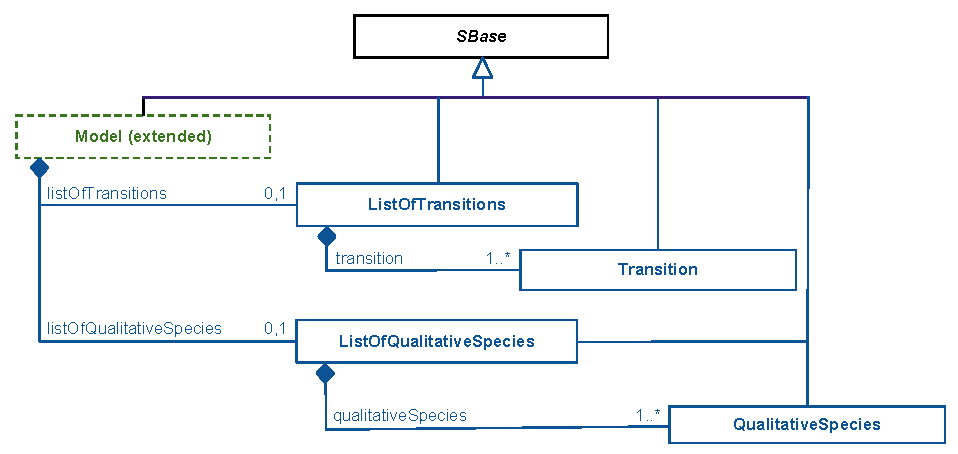
\includegraphics{figs/qual-extended-model-uml.pdf}
  \caption{The definitions of the extended \Model class. In other respects, \Model remains defined as
    in the SBML Level~3 Core specification.}
  \label{qual-extended-model-uml}
\end{figure}

\pagebreak
% -----------------------------------------------------------------------------
\subsection{The \class{QualitativeSpecies} class}
\label{qualSpecies-class}
Similarly to the \sbml{Species} in SBML, the components of qualitative models refer to pools of entities that are considered indistinguishable and are each located in a specific \sbml{Compartment}. However, here components are characterised by their qualitative influences rather than by taking part in reactions. Therefore, we define the \QualitativeSpecies element to represent such pools of entities.

\hl{In a Petri net, {\em qualitative species} refer to the places of the model, while in a logical model, they refer to the variables of this model (i.e. nodes of the influence graph).}

A \QualitativeSpecies describes a pool of indistinguishable entities in a \sbml{Compartment}. It is associated with  a \token{level} (an integer representing e.g. an activity state, or a functional level of concentration, etc)  %or a \token{symbolValue} from its \ListOfSymbolicValues.
 These objects classes are defined in \fig{qual-qualitative-species-uml}.
%\TODO{add listOfSymbols back}
\begin{figure}[h]
  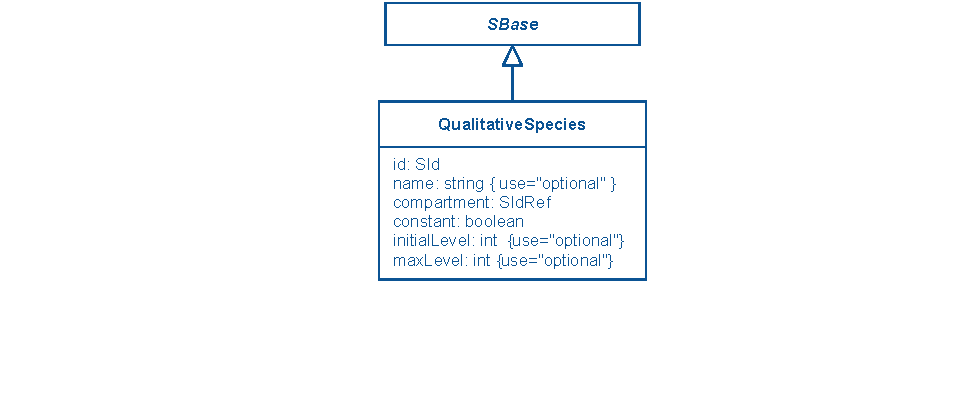
\includegraphics{figs/qual-qualitative-species-uml.pdf}
  \caption{The definitions of the \QualitativeSpecies class. }
  \label{qual-qualitative-species-uml}
\end{figure}

\paragraph{The \fixttspace\token{id} attribute}

The \token{id} attribute takes a required value
of type \primtype{SId}. The \token{id} is used as an identifier for the particular \QualitativeSpecies. It can be used as a 
<ci> element within MathML, in which case it it interpreted as the \emph{level} of this \QualitativeSpecies.

\paragraph{The \fixttspace\token{name} attribute}

A \QualitativeSpecies also has an optional \token{name} attribute of type \primtype{string}. 
 The \token{name} attribute should be used
in the same manner as on SBML Level~3 Core
objects; see Section~3.3.2 of the SBML Level~3 Version~1 Core
specification for more information.


\paragraph{The \token{compartment} attribute}
The required attribute \token{compartment}, of type \primtype{SIdRef}, is used to identify the compartment in which the qualitativeSpecies is located.  The attribute's value must be the identifier of an existing \sbml{Compartment} object in the model.  This attribute is comparable with the \token{compartment} attribute on the \sbml{Species} element.

\paragraph{The \token{constant} attribute}
The required attribute \token{constant}, of type \primtype{boolean}, is used to indicate that the \token{level} of the qualitativeSpecies is fixed or can be varied. This attribute is comparable with the \token{constant} attribute on the \sbml{Species} element.

Typically, in a regulatory or influence graph a \QualitativeSpecies may receive no interaction and if so, would appear only as an \Input in the model and have the value of the \token{constant} attribute set to \val{true}. In other influence graphs or in Petri Net models a \QualitativeSpecies may occur as an \Input whose level is changed by the \Transition and would have \token{constant} set to \val{false}.  The nature of changes to a \QualitativeSpecies resulting from a \Transition is also recorded using the \token{transitionEffect} attribute on the \Input (see section \ref{input-class}) and may be set to \val{none} to indicate there is no change. This duplication of information provides a means of validating the modeller's intent and also allows entities on the borders of a system to be easily identified.
 


\paragraph{The \token{initialLevel}  attribute}
The \token{initialLevel} is an \primtype{integer} that defines the initial \emph{level} of the \QualitativeSpecies in its \sbml{Compartment}. This attribute is optional but if set it cannot exceed the value of the \token{maxlevel} attribute, if this has been set.

\paragraph{The \token{maxLevel} attribute}
The \token{maxLevel} is an \const{integer} that sets the maximal \emph{level} of the \qualt{QualitativeSpecies}. This attribute is optional \textcolor{blue}{but when set, the \emph{level} of the \QualitativeSpecies must not exceed this value at any point in a simulation.}

\textcolor{blue}{In Petri nets, this attribute is meant to define place capacities. Hence, a transition is not enabled if the value resulting from its firing would exceed the  \token{maxLevel} of one of its output places. }

\textcolor{blue}{In logical models, the \token{maxLevel} should be coherent with the \token{resultLevel} values in the function terms defined for the corresponding transition, i.e. the model should not contain a \FunctionTerm that attempts to set a \emph{level} that exceeds this value.}

\textcolor{blue}{This attribute is can also be used to indicate the range of possible levels for a \QualitativeSpecies whose \token{constant} attribute is true. This may seem a little contradictory, since if the \token{constant} attribute is true then the level associated with the \QualitativeSpecies cannot vary. However, it provides additional information regarding the possible levels particularly in the case where no \token{initialLevel} has been set.}

%\subsubsection{The \class{SymbolicValue} class}
%The \QualitativeSpecies element may contain at most one \ListOfSymbolicValues that contains zero or more %\SymbolicValue elements. An empty list is allowed, and useful for e.g. adding annotations.
%
%The \SymbolicValue element defines a non instantiated parameter that allows the model to associate %undefined values with a particular \QualitativeSpecies.
%Symbols can be considered as uninstantiated parameters. Such symbols may represent the different %solutions of piecewise linear differential equations, along with different thresholds.
%
%\paragraph{The \token{id} attribute}
%A \SymbolicValue element has an \token{id} attribute that takes a required value
%of type \primtype{SId}. The \token{id} is used as an identifier for the particluar \SymbolicValue and may be %referenced by the \token{symbolicResult} attribute of a \FunctionTerm within a \Transition to indicate that %this \SymbolicValue is the resulting value for this \QualitativeSpecies following a particular \Transition.
%
%\paragraph{The \token{name} attribute}
%There is an optional \token{name} attribute of type \primtype{string} that should be used
%in the same manner as on SBML Level~3 Core
%objects; see Section~3.3.2 of the SBML Level~3 Version~1 Core
%specification for more information.
%
%
%\paragraph{The \token{rank} attribute}
%The \token{rank} is an \primtype{integer} that defines the position of the symbol in the \ListOfSymbolicValues. This attribute is optional. \Q{What difference does the position make or does rank meaning ordering independent of physical position ?}
%
%\Q{Are symbols and levels exclusive?}



% -----------------------------------------------------------------------------
\subsection{The \class{Transition} class}
\label{transitions-class}
A \Transition element contains at most one \ListOfInputs and one \ListOfOutputs and exactly one \ListOfFunctionTerms. These objects classes are defined in \fig{qual-transition-uml}.

\hl{The semantics of \Transition is that commonly used in Petri models, while in logical models, \Transition is used to specify the logical rule associated to a \QualitativeSpecies (that appears as an \Input of this \Transition). Hence, in principle, there is at most one \Transition defined for each component of the model. Note however, that input components, whose \token{constant} attribute is set to true, have no associated \Transition. }

\begin{figure}
  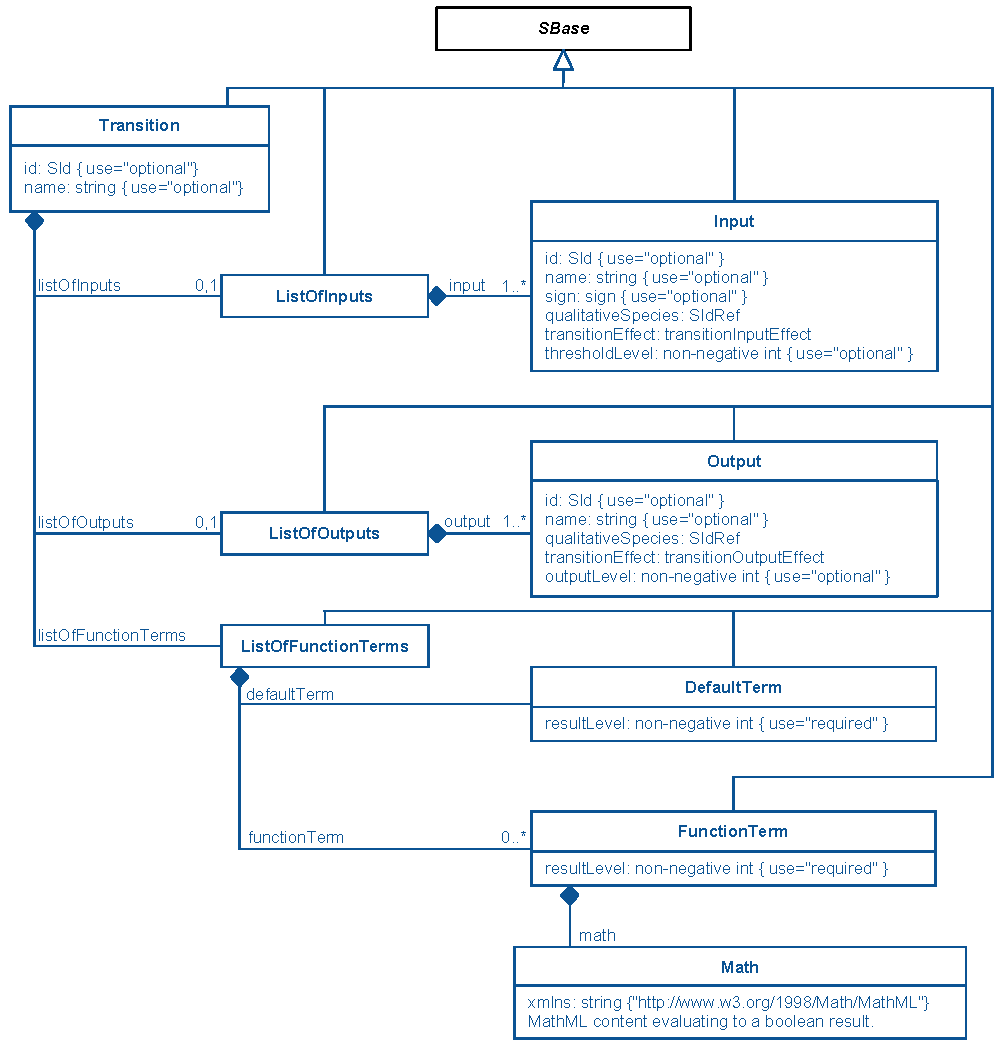
\includegraphics{figs/qual-transition-uml.pdf}
  \caption{The definitions of \Transition, \Input, \Output, \DefaultTerm and \FunctionTerm classes. Note that the \DefaultTerm class is not derived from SBase. }
  \label{qual-transition-uml}
\end{figure}

\paragraph{The \token{id} attribute}
A \Transition element has an optional \token{id} attribute of type \primtype{SId}.  In constrast to most SBML classes the \token{id} attribute on a \Transition has no mathematical interpretation.

\paragraph{The \token{name} attribute}
There is an optional \token{name} attribute of type \primtype{string} that should be used
in the same manner as on SBML Level~3 Core
objects; see Section~3.3.2 of the SBML Level~3 Version~1 Core
specification for more information.

%\paragraph{The \token{temporisationType} attribute}
%A \Transition has an attribute \token{temporisationType} of type \primtype{temporisationType} used to indicate the updating policy associated with this \Transition element. This attribute is optional. \tab{transition-temporisation} describes the different updating policies.
%
%\begin{table}[thb]
%  \begin{edtable}{tabular}{p{1in}p{5in}}
%    \toprule
%    \textbf{TemporisationType} & \textbf{Interpretation} \\
%    \midrule
%    \const{timer} & TBD \\
%    \const{priority} & TBD \\
%    \const{sustain} & TBD \\
%    \const{proportion} & TBD \\
%    \const{rate} & TBD \\
%    \bottomrule
%  \end{edtable}
%  \caption{Interpretation of the \token{temporisationType} attribute on a \Transition.} 
%  \label{transition-temporisation}
%\end{table}
%
%\TODO{need more explanation of this}

\subsubsection{The \class{Input} class}
\label{input-class}
\hl{The \ListOfInputs contains at least one element of type \Input. }
%A transition with zero inputs can be useful for defining an initial assignment, where the state of an output %depends on a function but not on any input values. An empty list is allowed, and useful for e.g. adding %annotations.
Each \Input refers to a \QualitativeSpecies that participates in the corresponding \Transition.
\hl{In Petri nets, these are the input places of the transition. In logical models, they are the regulators of the species whose behaviour is defined by the transition.}

\paragraph{The \token{id} attribute}
An \Input element has an optional \token{id} attribute of type \primtype{SId}. The identifier of an \Input can be used as a 
<ci> element within MathML, in which case it it interpreted as the \token{thresholdLevel}.

\paragraph{The \token{name} attribute}
There is an optional \token{name} attribute of type \primtype{string} that should be used
in the same manner as on SBML Level~3 Core
objects; see Section~3.3.2 of the SBML Level~3 Version~1 Core
specification for more information.


\paragraph{The \token{qualitativeSpecies} attribute}
The required attribute \token{qualitativeSpecies}, of type \primtype{SIdRef}, is used to identify the \QualitativeSpecies that is the \emph{input} of this \Transition.  The attribute's value must be the identifier of an existing \QualitativeSpecies object in the model.  This attribute is comparable with the \token{species} attribute on the \sbml{SpeciesReference} element.

\paragraph{The \token{thresholdLevel}  attribute}
The \token{thresholdLevel} is a \primtype{integer} that can be used to set the threshold level of the particular input. This attribute relates to the contribution of this input required for the transition to take place. In logical regulatory models, it refers to the threshold level above which the regulation takes place, while in a Petri net, it refers to the number of tokens required to enable to transition \hl{(weight of the arc connecting the input place to the transition). When defined, this attribute should be coherent with the content of the \FunctionTerm.}

\textcolor{blue}{The \token{thresholdLevel} is used by the FunctionTerms associated with the containing \Transition to determine the applicable \token{resultLevel} that should be applied. The \token{id} of the \Input represents this value and can be used in the \token{math} element of a \FunctionTerm. When defined, this attribute should be coherent with the content of the \FunctionTerm, {\em i.e.} if a \emph{number} is used in the \FunctionTerm to compare the current \emph{level} of a species, this number must correspond to the \token{thresholdLevel} of the corresponding \Input.}

\paragraph{The \token{transitionEffect} attribute}
Each \Input has a required attribute \token{transitionEffect} of type \primtype{transitionInputEffect} which describes how the \QualitativeSpecies referenced by the \Input is affected by the \Transition. \tab{transition-input} shows the possible values with the interpretation of each value.

\begin{table}[thb]
  \begin{edtable}{tabular}{p{1in}p{5in}}
    \toprule
    \textbf{TransitionInputEffect} & \textbf{Interpretation} \\
    \midrule
    \const{none} & The level associated with the \token{qualitativeSpecies} is not modified.\\
    \const{consumption} & The level of the \token{qualitativeSpecies} is decreased by the \token{resultLevel} of the selected term possibly modified by the \token{thresholdLevel} of the \Input.\\
    \bottomrule
  \end{edtable}
  \caption{Interpretation of the \token{transitionEffect} attribute on an \Input.} 
  \label{transition-input}
\end{table}

The following example illustrates the interpretation of the transitionEffect attribute. 

\begin{example}
<listOfInputs>
    <input qualitativeSpecies="A"   transitionEffect="none"        thresholdLevel="2" />
    <input qualitativeSpecies="B"   transitionEffect="consumption"/>
    <input qualitativeSpecies="C"   transitionEffect="consumption" thresholdLevel="2" />
</listOfInputs>
\end{example}

In the case of qualitativeSpecies \val{A} the \token{level} is unaltered by the \Transition and hence the \token{transitionEffect} attribute is set to \val{none}. 

The \token{level} of qualitativeSpecies \val{B} is reduced; hence the \token{transitionEffect} is \val{consumption}. The \token{level} is reduced by the value of the \token{resultLevel} from the whichever \FunctionTerm is applicable  (see \ref{sec:function-term}). 

Similarly, the \token{level} of \val{C} is also reduced, but on this occasion by $2$ (the \token{threholdLevel}) times the appropriate \token{resultLevel} . 

\hl{It should be noted that in logical models the \token{transitionEffect} is always set to \val{none}, while in Petri nets, it can be set to \val{none} (indicating a read arc) or to \val{consumption}. } The Petri net example in \ref{examples} provides further example of the use of the \token{transitionEffect} and \token{thresholdLevel} attributes. 

%\TODO{An example of a resultLevel modified by a thresholdLevel}

 
\paragraph{The \token{sign} attribute}
The \token{sign} of type \primtype{sign} can be used as an indication as to whether the contribution of this input is positive, negative, both (dual) or unknown. The sign is usually used for visualization purposes only. This attribute is optional.


\subsubsection{The \class{Output} class}
\label{output-class}

\hl{The \ListOfOutputs contains at least one element of type \Output. }
%A transition with zero outputs can be useful for modelling the effect of the environment. For example, in %Petri nets, a sink transition (with no output) will consume all tokens arriving in its input places; in logical %models, there should not be such transitions. 

\hl{Each \Output refers to a \QualitativeSpecies that participates in (is affected by) the corresponding \Transition. When a \Transition has several outputs, it is because the referenced species share the same regulators and the same logical rules.}


\hl{In a logical model, a \QualitativeSpecies should be referenced in at most one \ListOfOutputs, (that of the \Transition defining the evolution of this species). } \textcolor{blue}{This restriction is discussed in more detail in \ref{best-practices}}   


\paragraph{The \token{id} attribute}
An \Output element has an optional \token{id} attribute of type \primtype{SId}.  The identifier of an \Output can be used as a 
<ci> element within MathML, in which case it it interpreted as the \token{outputLevel}.

\paragraph{The \token{name} attribute}
There is an optional \token{name} attribute of type \primtype{string} that should be used
in the same manner as on SBML Level~3 Core
objects; see Section~3.3.2 of the SBML Level~3 Version~1 Core
specification for more information.



\paragraph{The \token{qualitativeSpecies} attribute}
The required attribute \token{qualitativeSpecies}, of type \primtype{SIdRef}, is used to identify the \QualitativeSpecies that is the \emph{output} of this \Transition.  The attribute's value must be the identifier of an existing \QualitativeSpecies object in the model.  This attribute is comparable with the \token{species} attribute on the \sbml{SpeciesReference} element.

\paragraph{The \token{outputLevel} attribute}
The \token{outputLevel} is an \primtype{integer} used along with the \token{transitionEffect} to specify the effect of the \Transition on the corresponding \QualitativeSpecies. This attribute is optional.  \hl{It has no use in logical models. In Petri nets, it relates to the weight of the arc connecting the transition to the output place.}

\paragraph{The \token{transitionEffect} attribute}
Each \Output has a required attribute \token{transitionEffect} of type \primtype{transitionOutputEffect} which describes how the \QualitativeSpecies referenced by the \Output is affected by the \Transition. \tab{transition-output} shows the possible values with the interpretation of each value.



\begin{table}[thb]
  \begin{edtable}{tabular}{p{1in}p{5in}}
    \toprule
    \textbf{TransitionOutputEffect} & \textbf{Interpretation} \\
    \midrule
    \const{production} & The level of the \token{qualitativeSpecies} is increased by the \token{resultLevel} of the selected term possibly modified by the \token{outputLevel} of the \Output.\\
    \const{assignmentLevel} & The level of the \token{qualitativeSpecies} is set to the \token{resultLevel} of the selected term. \\
%    \const{assignmentSymbol} & The symbol of the \token{qualitativeSpecies} is set to the \token{resultSymbol} of the selected term.\\
    \bottomrule
  \end{edtable}
  \caption{Interpretation of the \token{transitionEffect} attribute on an \Output.} 
  \label{transition-output}
\end{table}

The following example illustrates the interpretation of the transitionEffect attribute. In the case of qualitativeSpecies \val{A} the \token{level} is assigned the \token{resultLevel} from the whichever \FunctionTerm is applicable, whereas the \token{level} of qualitativeSpecies \val{B} is increased by \token{resultLevel}. Similarly, the \token{level} of \val{C} is increased by $2$ (\token{outputlevel}) times \token{resultLevel} (see also Petri net example in \ref{examples}). 

\begin{example}
<listOfOutputs>
    <output qualitativeSpecies="A"   transitionEffect="assignmentLevel"/>
    <output qualitativeSpecies="B"   transitionEffect="production"/>
    <output qualitativeSpecies="C"   transitionEffect="production"  outputLevel="2" />
</listOfInputs>
\end{example}

\textcolor{blue}{In logical models the \token{transitionEffect} is set to \val{assignmentLevel} whilst in standard PetriNets it is set to \val{production}.  It is envisioned that to encode High level PetriNets it will be necessary to allow the use of \val{assignmentLevel} as an \Output \token{transitionEffect}; however that is beyond the scope of the current specification.}

\subsubsection{The \ListOfFunctionTerms class}

The \ListOfFunctionTerms may contain any number of \FunctionTerm elements, and exactly one \DefaultTerm.  Each \FunctionTerm encodes the conditions under which this term is selected.  \hl{The \DefaultTerm describes the result of the \Transition applied by default ({\em i.e.} when no term evaluates to \val{true}). }

\subsubsection{The \DefaultTerm class}
\label{defaultTerm-class}
The \DefaultTerm defines the default result of a \Transition.  This term is used if there are no other \FunctionTerm elements or if none of the \sbml{Math} elements of the \FunctionTerm elements evaluates to \val{true}. 

\paragraph{The \token{resultLevel} attribute}
The default result is described by a \token{resultLevel}. This attribute is required.

The \token{resultLevel} is an \primtype{integer} describing a level.  The \token{resultLevel} is used; possibly together with the \token{thresholdLevel} or \token{outputLevel} to determine the level of a \QualitativeSpecies resulting from the \Transition. 

\subsubsection{The \class{FunctionTerm} class}
\label{sec:function-term}

Each \FunctionTerm is also associated with a result  and in addition to a Boolean function inside a \sbml{Math} element that can be used to set the conditions under which this term is selected.

\paragraph{The \token{resultLevel} attribute}
The result of the term is described by a the required attribute \token{resultLevel}.

The \token{resultLevel} is an \primtype{integer} describing a level.   The \token{resultLevel} is used; possibly together with the \token{thresholdLevel} or \token{outputLevel} to determine the level of a \QualitativeSpecies resulting from the \Transition. 

\paragraph{The \sbml{Math} element:}
Each \qual{FunctionTerm} holds a \primtype{boolean} function encoded in a \sbml{Math} element, using the subset of MathML 2.0 as defined in SBML L3v1 Section 3.4.6.
This element encodes the conditions under which the \FunctionTerm is selected. \hl{When the \sbml{Math} element contains the identifier of a \QualitativeSpecies, \Input or \Output, this identifier represents the level, \token{thresholdLevel} or \token{outputLevel} of the corresponding element. It should be noted that for the purposes of this specification these all have integer values. This specification does not preclude the use of these identifiers to represent \token{true} or \token{false}; however it is highly recommended that any the \token{math} element unambiguously returns a \primtype{boolean} function. Tools should take care to specify how integer values will be interpreted in relation to boolean constructs. }


\hl{\subsubsection{Mathematical interpretation of Transitions and FunctionTerms}}
\label{math-interpret}

\hl{In the Qualitative Models  package, {\em transitions} are the central mechanism for describing processes that change the levels of the qualitative species of the model. Here, we clarify their interpretation in the framework of logical modelling.}

\hl{The {\em function terms}  of a \Transition define the transition function one \QualitativeSpecies, {\em i.e.} its state transitions that depend on the levels of the species that appear as input of that transition (its "regulators"). The {\em function terms} together with the {\em default term} thus define a state transition table indicating what level the qualitative species will move to (target level), based on the current level of its regulators. In the case of multi-valued (as opposed to Boolean), this evolution proceeds step-wise towards the target level, {\em i.e.} each component of two successor states of the system differ at most by $1$. }\textcolor{blue}{The \QualitativeSpecies affected by the \Transition is referenced by the \Output element. In the situation where there is more than one \Output listed, the referenced species share the same regulators and the same logical rules.}

\hl{The model must be fully defined. Whatever the state of the system, one single value must apply (that of the \DefaultTerm or the \token{resultLevel} of a \FunctionTerm). More than one \FunctionTerm can share the same \token{resultLevel}, which is the equivalent to a single term holding the {\bf disjunction} (OR) of all these terms.  There should be no conflicting terms:  whenever multiple function terms apply (are true), their \token{resultLevel} should be the same. }

\textcolor{blue}{It should be noted that the \emph{level} associated with a \QualitativeSpecies has values from 0 up to the \token{maxLevel} (where declared). The mathematics of the model (i.e. the \FunctionTerm and \DefaultTerm element together with the \token{transitionEffect}) should not allow the {emph} level to either become negative or exceed the maximum.}

\hl{Importantly, given a model, one has then to choose an updating policy that defines how enabled transitions are processed (synchronously, asynchronously, etc.). However, this information is not part of the model {\em per se}. }




\subsection{Namespace scoping rules for identifiers}
\label{sec:ns-id}

The values of any \token{id} attribute  of type \primtype{SId} within the qual namespace are considered to have the same scope as the \token{id} attribute in the core SBML namespace. Thus the values of the attributes
  \token{id} and \token{qual:\-id} must be unique across the set of all \token{id} and
  \token{qual:\-id} attribute values of all objects in a model. In addition to those classes of objects specifed in the SBML Level 3 Version 1 Core specification;
  \Model, \FunctionDefinition, \Compartment,
  \Species, \Reaction, \SpeciesReference, \ModifierSpeciesReference,
  \Event, and \Parameter objects, this includes the following objects from this Qualitative Modelling package: \QualitativeSpecies, \Transition, 
  \Input and \Output.

% -*- TeX-master: "sbml-level-3-version-2-core"; fill-column: 66 -*-
% $Id: examples.tex 12140 2010-10-06 05:00:16Z mhucka $
% $HeadURL: https://svn.code.sourceforge.net/p/sbml/code/trunk/specifications/sbml-level-3/version-1/core/spec/examples.tex $
% ----------------------------------------------------------------

% Macros used in this section to provide common typesetting styles.

\newcommand{\species}[1]{\ensuremath{#1}\xspace}
\newcommand{\concent}[1]{\ensuremath{[#1\mkern1mu]}\xspace}
\newcommand{\unit}[1]   {\text{#1}\xspace}

\newcommand{\graybox}[1]{\colorbox[gray]{.85}{#1}}


\section{Example models expressed in XML using SBML}
\label{sec:xml-rep}
\label{sec:examples}

In this section, we present several examples of complete models
encoded in XML using SBML Level~3.


%-----------------------------------------------------------------------------
\subsection{A simple example application of SBML}
\label{sec:modeleg}
%-----------------------------------------------------------------------------

\newcommand{\kon} {\ensuremath{k_\text{on}}\xspace}
\newcommand{\koff}{\ensuremath{k_\text{off}}\xspace}
\newcommand{\kcat}{\ensuremath{k_\text{cat}}\xspace}

Consider the following representation of an enzymatic reaction:
\begin{center}
  \ce{\species{E} + \species{S} <=>[\kon][\koff] \species{ES} ->[\kcat] \species{E} + \species{P}}
\end{center}
In our model, we use the following initial species amounts:
\begin{larray*}
  \species{E}  &=& 5 \cdot 10^{-21} \; \unit{mole} \\
  \species{S}  &=& 10^{-20} \; \unit{mole} \\
  \species{P}  &=& 0 \; \unit{mole} \\ 
  \species{ES} &=& 0 \; \unit{mole}
\end{larray*}
Note that the species quantities are initialized in terms of
substance amounts rather than concentrations.  We also define the
following values for the kinetic constants:
\begin{larray*}
  \kon  &=& 1\:000\:000 \; \unit{litre} \; \unit{mole}^{\,-1} \; \unit{second}^{\,-1}\\
  \koff &=& 0.2 \; \unit{second}^{\,-1}\\
  \kcat &=& 0.1 \; \unit{second}^{\,-1}
\end{larray*}
We place everything in a single compartment we call ``comp'' whose
volume is $10^{-14}$ litres.  The following is a minimal but
complete SBML document encoding this model:

\sbmlexample{enzymekinetics.xml}

The model features local parameter definitions in each reaction.
In this case, the three parameters (\token{kon}, \token{koff},
\token{kcat}) all have unique identifiers and they could also have
just as easily been declared global parameters.  Local parameters
frequently become more useful in larger models, where it may
become tedious to assign unique identifiers for all the different
parameters.

The example above also demonstrates the use of unit specifications
throughout the model.  The \token{model} components define the
units of kinetic laws as being \unit{mole}/\unit{second} by virtue
of the values of the attributes \token{extentUnits} and
\token{timeUnits}.  In the rest of the model, species, parameters
and compartments are defined with appropriate units so that the
mathematical formulas inside the \token{kineticLaw} elements work
out to be \unit{mole}/\unit{second}.


%-----------------------------------------------------------------------------
\subsection{A simple example using the \token{conversionFactor} attribute}
\label{sec:eg:conversionfactor}
%-----------------------------------------------------------------------------

This example involves the same enzymatic reaction as in the
example of Section~\ref{sec:modeleg}:
\begin{center}
  \ce{\species{E} + \species{S} <=>[\kon][\koff] \species{ES} ->[\kcat] \species{E} + \species{P}}
\end{center}
In this new version of the model, we deliberately define the
species with different units from the unit of reaction extent in
the model.  This leads to two illustrative problems: (1) the
reaction rate expressions must be changed in order to reconcile
the differences between the species units and the unit of reaction
extent in the model, and (2) the formulas constructed for species'
rate-of-change equations must use conversion factors to reconcile
the differences between the units of the reaction rate expressions
and the units in which the species quantities are measured.

We begin with the following new \Species object definitions:
\begin{larray*}
  \species{E}   &=& 5 \cdot 10^{-18}\; \unit{millimole} \\
  \species{S}   &=& 10^{-17}\; \unit{millimole} \\
  \species{P}   &=& 0\; \unit{gram} \\
  \species{ES}  &=& 0\; \unit{millimole}
\end{larray*}
We keep the units of extent and time in the model the same as in
Example~\ref{sec:modeleg}; that is, the overall unit of extent in
the model is \unit{mole} and the unit of time is \unit{second},
set by assigning appropriate values to the attributes
\token{extentUnits} and \token{timeUnits}, respectively, on the
\Model object definition.  The differences between these and the
units of the species means that we have to adjust the reaction
rate expressions from their original versions in the model.  In
what follows, we illustrate one approach to doing so, and in
Section~\ref{sec:eg:conversionfactor2} we illustrate a second
approach.  The method in the present section involves changing the
values of the kinetic rate constants in the reaction rate
formulas, while the example of
Section~\ref{sec:eg:conversionfactor2} does not change the kinetic
constants but does require the introduction of additional
parameters.

\newcommand{\veq}    {\ensuremath{v_\text{veq}}\xspace}
\newcommand{\vcat}   {\ensuremath{v_\text{vcat}}\xspace}
\newcommand{\Vcomp}  {\ensuremath{V_\text{comp}}\xspace}
\newcommand{\convE}  {\ensuremath{c_\species{E}}\xspace}
\newcommand{\convS}  {\ensuremath{c_\species{S}}\xspace}
\newcommand{\convP}  {\ensuremath{c_\species{P}}\xspace}
\newcommand{\convES} {\ensuremath{c_{\species{ES}}}\xspace}
\newcommand{\konnew} {\ensuremath{k_\text{on}^{*}}\xspace}
\newcommand{\koffnew}{\ensuremath{k_\text{off}^{*}}\xspace}
\newcommand{\kcatnew}{\ensuremath{k_\text{cat}^{*}}\xspace}

The reaction rate formulas (\ie the formulas in the \token{math}
elements of \KineticLaw objects) were previously
\begin{larray}
  \label{eq:v1}
  \veq  &=& \Vcomp \cdot (\kon \cdot \concent{E} \cdot \concent{S} - \koff \cdot \concent{ES})\\
  \label{eq:v2}
  \vcat &=& \Vcomp \cdot \kcat \cdot \concent{ES}
\end{larray}
where \Vcomp stands for the size of compartment \val{comp} in the
SBML model.  Recalling the values of the parameters \kon, \koff,
and \kcat,
\begin{larray*}
  \kon  &=& 1\:000\:000 \; \unit{litre} \; \unit{mole}^{\,-1} \; \unit{second}^{\,-1}\\
  \koff &=& 0.2 \; \unit{second}^{\,-1}\\
  \kcat &=& 0.1 \; \unit{second}^{\,-1}
\end{larray*}
it becomes clear that, with the values of \species{E}, \species{S}
and \species{ES} all in \unit{millimoles}, Equations~\ref{eq:v1}
and~\ref{eq:v2} no longer lead to units of
\unit{mole}/\unit{second} for the reaction rates.  To compensate,
we change the values of the constants \kon, \koff, and \kcat using
the following simple transformations:
\begin{larray*}
  \konnew = & \kon \cdot \left( \dfrac{1 \; \unit{mole}}{1000 \; \unit{millimoles}} \right)^{2}
  & = 1 \; \unit{litre} \; \unit{mole} \; \unit{millimole}^{-2} \; \unit{second}^{\,-1} \\[4pt]
  \koffnew = & \koff \cdot \dfrac{1 \; \unit{mole}}{1000 \; \unit{millimoles}}
  & = 0.0002 \, \unit{mole} \; \unit{millimole}^{-1} \; \unit{second}^{\,-1} \\[4pt]
  \kcatnew = & \kcat \cdot \dfrac{1 \; \unit{mole}}{1000 \; \unit{millimoles}}
  & = 0.0001 \, \unit{mole} \; \unit{millimole}^{-1} \; \unit{second}^{\,-1}
\end{larray*}\vspace*{0.2ex}
The ``\unit{mole}/\unit{millimole}'' portion of the units are
admittedly unconventional for mass-action kinetic rate constants.
They are unlikely to correspond to values found in textbooks or
databases.  The logic of this approach is that in an actual
experimental situation, with the units of the species as given in
the model (presumably representing how the species are being
measured), the kinetic rate constants are likely to be measured in
terms of the units above.  However, if that is not the case, then
the approach of Section~\ref{sec:eg:conversionfactor2} may be more
appropriate.

\newcommand{\nS}{\ensuremath{n_{\mkern-1muS}}\xspace}
\newcommand{\nP}{\ensuremath{n_{\mkern-1muP}}\xspace}

Taking these new \konnew, \koffnew and \kcatnew parameters and
replacing the original parameters in the reaction rate equations
finally leads to the following:
\begin{larray}
  \label{eq:veq-star}
  \veq  &=& \Vcomp \cdot (\konnew \cdot \concent{E} \cdot \concent{S} - \koffnew \cdot \concent{ES})\\
  \label{eq:vcat-star}
  \vcat &=& \Vcomp \cdot \kcatnew \cdot \concent{ES}
\end{larray}
Next, we turn to the rates-of-change equations for the species.
There are two cases: species \species{S}, whose unit of substance
is \unit{millimole}, and species \species{P}, whose unit of
substance is \unit{gram}.  We use SBML Level~3's conversion factor
mechanism to effectuate the necessary transformations, following
the guidelines described in Section~\ref{sec:about-kinetic-laws}.
In the model text below, we define a default conversion factor by
setting the value of the \Model object's \token{conversionFactor}
attribute to a parameter whose values is
\begin{linenomath}
  \begin{equation*}
    \dfrac{1000 \; \unit{millimole}}{1 \; \unit{mole}}
  \end{equation*}
\end{linenomath}
Let \csg stand for the \Model object's \token{conversionFactor}
attribute with the value above.  The rate-of-change equation for
\species{S} is the following:
\begin{linenomath}
  \begin{equation}\label{eq:dns}
    \dfrac{d \nS}{d t} = - \csg \cdot \graybox{$\Vcomp \cdot
    (\konnew \cdot \concent{E} \cdot \concent{S} - \koffnew \cdot \concent{ES})$}
  \end{equation}
\end{linenomath}
The portion inside the gray box in Equation~\ref{eq:dns} is simply
Equation~\ref{eq:veq-star}, and its value will have the unit
mole/second.  Multiplying this by \csg will produce a result in
millimole/second.  The stoichiometry of species \species{S} in the
reaction is \val{1}, but it is a reactant, thus the need for the
negative sign.

For species \species{P}, we need a different conversion factor, to
convert between the units of \unit{gram} and \unit{mole}.  We
accomplish this by setting a value for the \Species object's
\token{conversionFactor} attribute.  By virtue of being defined on
the \Species object for \species{P}, this conversion factor value
overrides the global value defined on the \Model object.  Let
\convP represent this conversion factor.  The equation for the
rate-of-change of \species{P} is the following:
\begin{linenomath}
  \begin{equation}\label{eq:dnp}
    \dfrac{d \nP}{d t} = \convP \cdot \graybox{$\Vcomp \cdot \kcatnew \cdot \concent{ES}$}
  \end{equation}
\end{linenomath}
The portion inside the gray box in Equation~\ref{eq:dnp} is simply
Equation~\ref{eq:vcat-star}, with a value in mole/second.
Multiplying by the conversion factor \val{convertToGram} defined
in the model below will yield gram/second.  The species
\species{P} is a product, and its stoichiometry is \val{1}; thus,
the right-hand side has a positive sign.

The following is the SBML encoding of this model:

\sbmlexample{conversionfactor1.xml}


%-----------------------------------------------------------------------------
\subsection{An alternative formulation of the \token{conversionFactor} example}
\label{sec:eg:conversionfactor2}
%-----------------------------------------------------------------------------

Here we present an alternative formulation of the model from the
previous section.  Once again, it involves the same enzymatic
reaction as in the example of Section~\ref{sec:modeleg}:
\begin{center}
  \ce{\species{E} + \species{S} <=>[\kon][\koff] \species{ES} ->[\kcat] \species{E} + \species{P}}
\end{center}
As in Section~\ref{sec:eg:conversionfactor}, we define the overall
unit of extent on the model to be \unit{mole} and the unit of time
to be \unit{second}; this means the unit of reaction rates is
\unit{mole}/\unit{second} as before.  We also set the initial
amounts and units as in the previous section:
\begin{larray*}
  \species{E}   &=& 5 \cdot 10^{-18} \; \unit{millimole} \\
  \species{S}   &=& 10^{-17} \; \unit{millimole} \\
  \species{P}   &=& 0 \; \unit{gram} \\
  \species{ES}  &=& 0 \; \unit{millimole}
\end{larray*}
Unlike in the previous section's model, however, here we retain
the values of the kinetic constants as they were originally in the
model of Section~\ref{sec:modeleg}:
\begin{larray*}
  \kon  &=& 1\:000\:000 \; \unit{litre} \; \unit{mole}^{\,-1} \; \unit{second}^{\,-1}\\
  \koff &=& 0.2 \; \unit{second}^{\,-1}\\
  \kcat &=& 0.1 \; \unit{second}^{\,-1}
\end{larray*}
We take a different approach to adjusting the reaction rate
expressions to account for the fact that the concentrations of the
species as they appear in the \KineticLaw elements are in units of
\unit{millimole}/\unit{litre}, while the unit of reaction extent
is \unit{mole} and reaction rates are in
\unit{mole}/\unit{second}.  Our approach here is to introduce
constants into the reaction rate expressions to convert the
substance units to \unit{mole} and multiply each occurence of a
concentration by that constant.  A separate constant is necessary
for each \Species object appearing in a \KineticLaw object,
although it turns out that in the particular situation under
consideration here, the constants are all identical:
\begin{linenomath}
  \begin{equation*}
      \convE = \convS = \convES = 10^{-3} \; \unit{mole} \; \unit{millimole}^{\,-1}
  \end{equation*}
\end{linenomath}
Applying this approach, the reaction rate equations become the
following:
\begin{larray*}
  \veq  &=& \Vcomp \cdot (\kon \cdot \concent{E} \cdot \convE \cdot \concent{S} \cdot \convS
  - \koff \cdot \concent{ES} \cdot \convES)\\
  \vcat &=& \Vcomp \cdot \kcat \cdot \concent{ES} \cdot \convES
\end{larray*}
where again \Vcomp stands for the size of compartment called
\val{comp} in the SBML model.  We construct the rate-of-change
equations for the each species using the guidelines described in
Section~\ref{sec:about-kinetic-laws}, and in this case, the
equations for species \species{S} and \species{P} are
\begin{larray*}
  \dfrac{d \nS}{d t} &=& - \csg \cdot \Vcomp \cdot
  (\kon \cdot \concent{E} \cdot \convE \cdot \concent{S} \cdot \convS
  - \koff \cdot \concent{ES} \cdot \convES) \\[5pt]
  \dfrac{d \nP}{d t} &=& \convP \cdot \Vcomp \cdot \kcat \cdot \concent{ES} \cdot \convES
\end{larray*}
where again \csg stands for the value of the \Model object's
\token{conversionFactor} attribute and \convP is the value of the
\token{conversionFactor} attribute of the \Species object
definition for \species{P}.

The SBML encoding of this model is given below:

\sbmlexample{conversionfactor2.xml}


%-----------------------------------------------------------------------------
\subsection{Example of a discrete version of a simple dimerization reaction}
\label{sec:discrete-eg}
%-----------------------------------------------------------------------------

\emph{(SBO annotations for this model contributed by Lukas Endler,
  EMBL-EBI, Cambridge, UK.)}

This example illustrates subtle differences between models
formulated for use in a continuous simulation framework (\eg using
differential equations) and those intended for a discrete
simulation framework.  The model shown here is suitable for use
with a discrete stochastic simulation algorithm of the sort
developed by \cite{gillespie:1977}.  In such an approach, species
are described in terms of molecular counts and simulation
proceeds by computing the probability of the time and identity of
the next reaction, then updating the species amounts
appropriately.

The model involves a simple dimerization reaction for a protein
named \species{P}:
\begin{linenomath}
\begin{equation*}
    2 P  \leftrightarrow  P_2
\end{equation*}
\end{linenomath}
The SBML representation is shown below.  There are several notable
points.  First, species \species{P} and \species{P_2} (represented
by \val{P} and \val{P2}, respectively) are declared to be always
in terms of discrete amounts by using the flag
\token{hasOnlySubstanceUnits}=\val{true} on the \Species object
definitions.  This indicates that when the species identifiers
appear in mathematical formulas, their values have units of
\quantity{substance amount}, not \{\quantity{substance
  amount}\}/\quantity{size}.  A second point is that, as a result,
the corresponding \KineticLaw formulas do not need volume
corrections.  In Gillespie's approach, the constants in the rate
expressions (here, $c_1$ and $c_2$, represented in the SBML model
by \token{c1} and \token{c2}, respectively) contain a contribution
from the kinetic constants of the reaction and the size of the
compartment in which the reactions take place.  This is a
convention commonly adopted by stochastic modelers, but is in no
way essential---it is perfectly reasonable to factor volume out of
the rate constants, and in certain situations it may be desirable
to do so (\eg for models having time-varying compartment volume),
but due to the use of substance units, it must be done differently
compared to the deterministic case.  Third, although the reaction
is reversible, it is encoded as two separate irreversible
reactions, one each for the forward and reverse directions, as
averaging over the reactions will affect the stochasticity.
Finally, note that the rate expression for the forward reaction is
a second-order mass-action reaction, but it is the \emph{discrete}
formulation of such a reaction rate~\citep{gillespie:1977}.

\sbmlexample{dimerization.xml}

This example also illustrates the need to provide additional
information in a model so that software tools using different
mathematical frameworks can properly interpret it.  In this case,
a simulation tool designed for continuous ODE-based simulation
would likely misinterpret the model (in particular the reaction
rate formulas), unless it deduced that a discrete stochastic
simulation was intended.  One of the purposes of SBO annotations
(Section~\ref{sec:sboTerm}) is to enable such interpretation
without the need for deduction. However, the interpretation of the
model is essentially the same irrespective of whether the model is
to be simulated in a deterministic or stochastic manner, and a
properly SBML-compliant deterministic simulator will in most cases
correctly simulate the continuous deterministic approximation
of the stochastic model even if it has no stochastic simulation
capability.

\clearpage 

The interpretation of rate laws for stochastic models is similar
to, yet different from, that of deterministic models. Taking the
first reaction as an example, the rate law is $c_1P(P-1)/2$ reaction
events per second. In the continuous deterministic case, the
interpretation of this is that the extent of the reaction in time
$dt$ is $[c_1P(P-1)/2]dt$ (and this leads naturally to the usual ODE
formulation of the model). In the stochastic case, the
interpretation is that the \emph{propensity} (or \emph{rate}, or
\emph{hazard}) of the reaction is $c_1P(P-1)/2$. That is, the
\emph{probability} of a single reaction event occurring in time
$dt$ is $[c_1P(P-1)/2]dt$ (and note that the \emph{expected} extent of
the reaction will be $[c_1P(P-1)/2]dt$). This interpretation leads to a Markov
jump process for the system dynamics, where the inter-event times
are exponentially distributed. Such dynamics can be simulated
using a discrete event simulation algorithm such as the
\emph{Gillespie algorithm}. In this case, the algorithm for
simulating the model can be described as follows:

\begin{enumerate}

\item Initialize $t:=0,\ c_1:=0.00166,\ c_2:=0.2,\ P:=301,\ P_2:=0$

\item Compute $h_1:=c_1P(P-1)/2,\ h_2:=c_2P_2$

\item Compute $h_0=h_1+h_2$

\item Simulate $t'\sim \operatorname{Exp}(h_0)$ and set $t:=t+t'$

\item With probability $h_1/h_0$ set $P:=P-2,\ P_2:=P_2+1$,
  otherwise set $P:=P+2,\ P_2:=P_2-1$.

\item Output $t,\ P,\ P_2$

\item If $t<T_{max}$, return to step 2, otherwise stop.

\end{enumerate}

Although this is a simulation algorithm is a very practical way of
describing how to construct exact realizations of the Markov jump
process corresponding to the discrete stochastic kinetic model, it
is not a concise mathematical description. Such a description can
be provided by writing the model as a time change of a pair of
independent unit Poisson processes. Let $N_1(t)$ and $N_2(t)$ be
the counting functions of these processes, so that for each
$i=1,2$, $t>0$, $N_i(t)\sim \operatorname{Poisson}(t)$. Then,
writing $P(t)$ and $P_2(t)$ for the numbers of molecules of $P$
and $P_2$ at time $t$, respectively, we have that the stochastic process
$\{P(t),P_2(t)\,|\,t>0\}$ satisfies the stochastic integral equation
\begin{larray*}
  P_2(t) &=& N_1\left(\int_0^t
    c_1\frac{P(\tau)[P(\tau)-1]}{2}d\tau\right) - N_2\left(\int_0^t
    c_2 P_2(\tau)d\tau\right) \\[2pt]
  P(t) &=& 301 - 2P_2(t).
\end{larray*}
The above representation is arguably the most useful for
mathematical analysis of the stochastic model; see \cite{ball:2006} for
details. Another popular representation is the so-called chemical
Master equation (CME) for the probability distribution of the possible
states at all times \citep{gillespie:1992}. In this case, since there are
151 possible states of the system (corresponding to the 151
possible values of $P_2$), the CME consists of 151 coupled
ODEs,
\begin{linenomath}
  \begin{equation*}
    \frac{d}{dt}p(P,P_2,t) =
    \left\{
      \begin{array}{ll}
        \displaystyle-\frac{c_1}{2}\times 301\times 299p(301,0,t)+c_2p(299,1,t),
        & P=301,\ P_2=0,\\[10pt]
        \displaystyle\frac{c_1}{2}(P+2)(P+1)p(P+2,P_2-1,t)-\frac{c_1}{2}P(P-1)p(P,P_2,t) & P=301-x,\ P_2=x,\\[5pt]
        \qquad+c_2(P_2+1)p(P-2,P_2+1,t)-c_2P_2p(P,P_2,t),
        & \quad x=1,2,\ldots,149,\\[10pt]
        \displaystyle\frac{c_1}{2}\times 2\times 3p(3,149,t)-c_2\times 150p(1,150,t),
        & P=1,\ P_2=150,
      \end{array}
    \right.
  \end{equation*}
\end{linenomath}
where $p(P,P_2,t)$ denotes the probability that there are $P$
molecules of $P$ and $P_2$ molecules of $P_2$ at time $t$, and the
ODEs are subject to the initial conditions
\begin{linenomath}
  \begin{equation*}
    p(301,0,0)=1,\ p(301-2x,x,0)=0,\ x=1,2,\ldots,150.
  \end{equation*}
\end{linenomath}
See \cite{evans:2008} for further examples of discrete stochastic
kinetic models encoded in SBML and \cite{wilkinson_2006} for an
introduction to discrete stochastic modeling using SBML.



%-----------------------------------------------------------------------------
\subsection{Example involving assignment rules}
\label{apdx:rules-eg}
%-----------------------------------------------------------------------------

This section contains a model that simulates a system containing a
fast reaction.  This model uses rules to express the mathematics
of the fast reaction explicitly rather than using the \token{fast}
attribute on a reaction element.  The system modeled is
\begin{larray*}
  X_0 & \overset{\underrightarrow{k_1 [X_0]}}{}           & S_1 \\[6pt]
  S_1 & \overset{\underleftrightarrow{k_f [S_1] - k_r [S_2]}}{} & S_2 \\[6pt]
  S_2 & \overset{\underrightarrow{k_2 [S_2]}}{}           & X_1
\end{larray*}\vspace*{-1em}
\begin{larray*}
  k_1 = 0.1, \quad k_2 = 0.15, \quad k_f = K_{eq} 10000, \quad k_r = 10000, \quad K_{eq} = 2.5.
\end{larray*}
where $[X_0]$, $[X_1]$, $[S_1]$, and $[S_2]$ are species in
concentration units, and $k_1$, $k_2$, $k_f$, $k_r$, and $K_{eq}$
are parameters.  This system of reactions can be approximated with
the following new system:
\begin{larray*}
  X_0 & \overset{\underrightarrow{k_1 [X_0]}}{} & T \\[6pt]
  T   & \overset{\underrightarrow{k_2 [S_2]}}{} & X_1
\end{larray*}\vspace*{-1.5em}
\begin{larray*}
  [S_1] &=& \dfrac{[T]}{1 + K_{eq}} \\[6pt]
  [S_2] &=& K_{eq} [S_1]
\end{larray*}

where $T$ is a new species.  The following example SBML model
encodes the second system.

\sbmlexample{assignmentrules.xml}


%-----------------------------------------------------------------------------
\subsection{Example involving algebraic rules}
\label{sec:algeraiceg}
%-----------------------------------------------------------------------------

This section contains an example model that contains two
\AlgebraicRule objects that are necessary to determine the values
of two variables within the model.  In this particular case, the
rules cannot be rewritten in terms of \AssignmentRule.  This
example illustrates a more rigorous analysis of the enzymatic
reaction given in the example of Section~\ref{sec:modeleg}.
\begin{center}
  \ce{\species{E} + \species{S} <=>[k1_{\text{on}}][k1_{\text{off}}] \species{ES} ->[k2] \species{E} + \species{P}}
\end{center}
In this example, we describe a quasi-steady-state approximation of
the enzymatic reaction equation shown above.  It is based on two
assumptions.  First, the rate at which the concentration of the
substrate bound enzyme (\concent{ES}) changes is assumed to be
slow compared to the rate of change of concentration of both the
substrate (\concent{S}) and product (\concent{P}).  Second, the
total concentration of the enzyme is assumed to stay constant over
time.  This means we can assume the concentration of \concent{ES}
and \concent{E} are not governed by the reactions, and so some
other equations must be used to determine the values of these
concentrations in order to be able to simulate the model.

Applying the first assumption means that the rate of change of
\concent{ES} should be set to zero:
\begin{linenomath}
\begin{equation*}
  \dfrac{d \concent{ES}}{d t} = k1\sub{on} \cdot \concent{E} \cdot \concent{S}
     - (k1\sub{off} + k2) \cdot \concent{ES} = 0
\end{equation*}
\end{linenomath}

The second assumption can be written as
\begin{linenomath}
\begin{equation*}
  \concent{E\sub{total}} = \concent{E} + \concent{ES}
\end{equation*}
\end{linenomath}
which, after rearranging, becomes
\begin{linenomath}
\begin{equation*}
  \concent{E\sub{total}} - (\concent{E} + \concent{ES}) = 0
\end{equation*}
\end{linenomath}

Thus, we have two algebraic rules that must be applied to
determine the values of \concent{E} and \concent{ES}.  The SBML
encoding of this model is given below.  Note that the species
\species{E} and \species{ES} have their \token{boundaryCondition}
attribute set to \val{true}.  This means that a simulation tool
should not construct equations for them based on the reactions in
the system.  Their values are instead set using the rules in the
model.  Also, the model uses a dummy species
\species{E\sub{total}} with its \token{constant} attribute set to
\val{true}; its role is to assign the total concentration of the
enzyme in the model.  This could just as easily have been done
using a parameter instead of a constant dummy species, but we use
the latter approach as an illustration.

\sbmlexample{twoalgebraicrules.xml}


%-----------------------------------------------------------------------------
\subsection{Example with combinations of
  \token{boundaryCondition} and \token{constant} values on \class{Species}
  with \class{RateRule} objects}
\label{sec:constantspecieseg}
%-----------------------------------------------------------------------------

In this section, we discuss a model that includes four species,
each with a different combination of values for their
\token{boundaryCondition} and \token{constant} attributes.  The
model represents a hypothetical system containing one reaction,
\begin{linenomath}
\begin{equation*}
  \begin{array}{@{}ccc@{}}
    S_1 + S_2 & \overset{\underrightarrow{k_1 [S_1] [S_2] [S_3]}}{} & S_4 \\ \\[-4pt]
  \end{array}
\end{equation*}
\end{linenomath}
where \species{S_3} is a species that catalyzes the conversion of
species \species{S_1} and \species{S_2} into \species{S_4}.
Species \species{S_1} and \species{S_2} are on the boundary of the
system (\ie \species{S_1} and \species{S_2} are reactants but
their values are not determined by kinetic laws).  The value of
\species{S_1} in the system is determined over time by the rate
rule:
\begin{linenomath}
  \begin{equation*}
    \dfrac{d \concent{S_1}}{d t} = k_2
  \end{equation*}
\end{linenomath}
The species \species{S_2} and \species{S_3} are not affected by
the either the reaction or the rate rule, and have the following
initial concentration values:
\begin{linenomath}
  \begin{equation*}
    \concent{S_2} = 1, \quad \concent{S_3} = 2
  \end{equation*}
\end{linenomath}
The values of constant parameters in the system are:
\begin{linenomath}
  \begin{equation*}
    k_1 = 0.5, \quad k_2 = 0.1
  \end{equation*}
\end{linenomath}
and the initial values of varying species are:
\begin{linenomath}
  \begin{equation*}
    \concent{S_1} = 0, \quad \concent{S_4} = 0
  \end{equation*}
\end{linenomath}

The value of \concent{S_1} varies over time and it is on the
boundary, so in the SBML representation, \token{S1} has a
\token{constant} attribute with a value of \val{false} and a
\token{boundaryCondition} attribute with a value of \val{true}.
The value of $\concent{S_2}$ is fixed and it is also on the
boundary, so \token{S2} has a \token{constant} attribute value of
\val{false} and a \token{boundaryCondition} attribute value of
\val{true}.  $\concent{S_3}$ is fixed but not on the boundary, so
the \token{constant} attribute is \val{true} and the
\token{boundaryCondition} attribute is \val{false}.  Finally,
$\concent{S_4}$ is a product whose value is determined by a
kinetic law and therefore in the SBML representation has
\val{false} for both its \token{boundaryCondition} and
\token{constant} attributes.

The following is the SBML rendition of the model shown above:

\sbmlexample{boundarycondition.xml}


%-----------------------------------------------------------------------------
\subsection{Example of translation from a multi-compartmental model to ODEs}
\label{sec:odeeg}
%-----------------------------------------------------------------------------

This section contains a model with two compartments and four
reactions.  The model is derived from Lotka-Volterra, with the
addition of a reversible transport step.  When observed in a
time-course simulation, three of this model's species display
damped oscillations.

\begin{figure}[htb]
  \vspace*{5pt}
  \centering
  \begin{picture}(260,60)
    \put(0,10){\framebox(255,50)[tl]{ cytosol}}
    \put(10,19){\framebox(105,29)[tl]{ nucleus}}
    \put(24,26){$
        X + Y_{1n} \yields^{\cit k\sub{1}} 2\,Y_{1n}
        \eqbm^{\cit K\sub{T}} 2\,Y_{1c} + 2\,Y_2
        \yields^{\cit k\sub{2}} 4\,Y_2 \yields^{\cit k\sub{3}} \emptyset
        $}
  \end{picture}
  \vspace*{-8pt}
  \caption{An example multi-compartmental model.}
  \label{fig:multicomp}
\end{figure}

Figure~\ref{fig:multicomp} illustrates the arrangement of
compartments and reactions in the model
\token{LotkaVolterra\_transport}.  The reaction between the
compartments called \token{cytosol} and \token{nucleus} is a
transport reaction whose mechanisms are not modeled here; in
particular, the reaction does not take place on the membrane
between the compartments, and is modeled here simply as a process
that spans the two three-dimensional compartments.

The text of the SBML representation of the model is shown below,
and it is followed by its complete translation into ordinary
differential equations.  As usual, in this SBML model, the
reaction rate equations in the kinetic laws are in substance per
time units.  The reactions have also been simplified to reduce
common stoichiometric factors in the original system depicted in
Figure~\vref{fig:multicomp}.  The species variables in this SBML
representation are in concentration units; their initial
quantities are declared using the attribute \token{initialAmount}
on the \token{species} definitions, but since the attribute
\token{hasOnlySubstanceUnits} is \emph{not} set to true, the
identifiers of the species represent their concentrations when
those identifiers appear in mathematical expressions elsewhere in
the model.  Note that the species whose identifier is \val{X} is a
boundary condition, as indicated by the attribute
\token{boundaryCondition}=\val{true} in its definition.

\sbmlexample{multicomp.xml}

The ODE translation of this model is as follows.  First, we give
the values of the constant parameters:
\begin{larray*}
  k_1   &=& 2500\; \unit{litre} \; \unit{mole}^{\,-1}\; \unit{second}^{\,-1}\\
  k_2   &=& 2500\; \unit{litre} \; \unit{mole}^{\,-1}\; \unit{second}^{\,-1}\\
  K_3   &=& 25000\; \unit{second}^{\,-1}\\
  K_T   &=& 25000\; \unit{second}^{\,-1}
\end{larray*}
Now on to the initial conditions of the variables.  In the
following, the terms $[X]$, $[Y_{1n}]$, $[Y_{1c}]$, and $[Y_2]$
refer to the species' concentrations.  Note that the corresponding
species identifiers \token{X}, \token{Y\_{1n}}, \token{Y\_{1c}}
and \token{Y\_2} in the model are in concentration units, even
though all the values in the model are initialized in terms of
amounts.  (The reason the species identifiers in the model are
still in concentration units goes back to the meaning of the
\token{hasOnlySubstanceUnits} attribute on a \Species; if the
attribute is set to a value of \val{false}, a species' symbol in a
model is interpreted as a concentration or density regardless of
whether its initial value is set using \token{initialAmount} or
\token{initialConcentration}.)  We use $V_n$ to represent the size
of compartment \val{nucleus} and $V_c$ the size of compartment
\val{cytoplasm}:
\begin{larray*}
  V_n    &=& 1\; \unit{litre}\\
  V_c    &=& 5\; \unit{litre}\\
  X      &=& 1\; \unit{mole}\\
  Y_{1n} &=& 1\; \unit{mole}\\
  Y_{1c} &=& 0\; \unit{mole}\\
  Y_2    &=& 1/5\; \unit{mole}
\end{larray*}
And finally, here are the differential equations:
\begin{linenomath}
  \begin{align*}
    \dfrac{d [X]}{d t}    &= 0 \\[6pt]
    V_n \dfrac{d [Y_{1n}]}{d t} &= k_1 [X] [Y_{1n}] [V_n] - K_T \big([Y_{1n}] - [Y_{1c}]\big) V_c
    && \text{reactions production and transport} \\[6pt]
    V_c \dfrac{d [Y_{1c}]}{d t} &= K_T \big([Y_{1n}] - [Y_{1c}]\big) V_c - k_2 [Y_{1c}] [Y_2] V_c
    && \text{reactions transport and transformation} \\[6pt]
    V_c \dfrac{d [Y_2]}{d t}    &= k_2 [Y_{1c}] [Y_2] V_c - k_3 [Y_2] V_c
    && \text{reactions transformation and degradation}
  \end{align*}
\end{linenomath}
As formulated here, this example assumes constant volumes.  If the
sizes of the compartments \val{cytoplasm} or \val{nucleus} could
change during simulation, then it would be preferable to use a
different approach to constructing the differential equations.  In
this alternative approach, the ODEs would compute substance change
rather than concentration change, and the concentration values
would be computed using separate equations.  This approach is used
in Section~\ref{sec:about-kinetic-laws}.


%-----------------------------------------------------------------------------
\subsection{Example involving function definitions}
\label{sec:functioneg}
%-----------------------------------------------------------------------------

This section contains a model that uses the function definition
feature of SBML.  Consider the following hypothetical system:
\begin{linenomath}
\begin{equation*}
  \begin{array}{@{}ccc@{}}
    S_1 & \overset{\underrightarrow{f([S_1])}}{} & S_2 \\ \\[-4pt]
  \end{array}
\end{equation*}
\end{linenomath}
where
\begin{linenomath}
\begin{equation*}
    f(x) = 2 x
\end{equation*}
\end{linenomath}

The following is the XML document that encodes the model shown
above:

\sbmlexample{functiondef.xml}


%-----------------------------------------------------------------------------
\subsection{Example involving \emph{delay} functions}
\label{sec:delayeg}
%-----------------------------------------------------------------------------

The following is a simple model illustrating the use of $delay$ to
represent a gene that suppresses its own expression.  The model
can be expressed in a single rule:
\begin{linenomath}
\begin{equation*}
  \frac{d [P]}{d t} = \dfrac{ \dfrac{1}{1 + m [P_{delayed}]^q} - [P] }{ \tau }\\
\end{equation*}
\end{linenomath}
\vspace*{-0.5em}
where
\vspace*{-1em}
\begin{larray*}
  [P_\text{delayed}] && \text{is } delay([P], \Delta_t) \text{ or [P] at } t - \Delta_t\\[-2pt]
  [P]           && \text{is protein concentration}\\[-2pt]
  \tau          && \text{is the response time}\\[-2pt]
  m             && \text{is a multiplier or equilibrium constant}\\[-2pt]
  q             && \text{is the Hill coefficient}
\end{larray*}
and the species quantities are in concentration units.
The text of an SBML encoding of this model is given below:

\sbmlexample{delay.xml}


%-----------------------------------------------------------------------------
\subsection{Example involving events}
\label{sec:eventeg}
%-----------------------------------------------------------------------------

This section presents a simple model system that demonstrates the
use of events in SBML.  Consider a system with two genes,
$G_1$ and $G_2$.  $G_1$ is initially
on and $G_2$ is initially off.  When turned on, the two
genes lead to the production of two products, $P_1$ and $P_2$,
respectively, at a fixed rate.  When $P_1$ reaches a given
concentration, $G_2$ switches on.  This system can be
represented mathematically as follows:
\begin{linenomath}
\begin{eqnarray*}
  \dfrac{d [P_1]}{d t} & = & k_1 \big([G_1] - [P_1]\big)\\[3pt]
  \dfrac{d [P_2]}{d t} & = & k_2 \big([G_2] - [P_2]\big)\\[0pt]
  [G_2] & = &
    \begin{cases}
      0 & \text{when $[P_1] \leq \tau$},\\
      1 & \text{when $[P_1] > \tau$}.
    \end{cases}
\end{eqnarray*}
\end{linenomath}

The initial values are:
\begin{linenomath}
\begin{equation*}
  [G_1] = 1, \quad [G_2] = 0, \quad \tau = 0.25, \quad P_1 = 0, \quad P_2 = 0, \quad k_1 = k_2 = 1.
\end{equation*}
\end{linenomath}

The SBML Level 3 representation of this is as follows:

\sbmlexample{events.xml}


%-----------------------------------------------------------------------------
\subsection{Example involving two-dimensional compartments}
\label{sec:two-dimensional-eg}
%-----------------------------------------------------------------------------

The following example is a model that uses a two-dimensional
compartment.  It is a fragment of a larger model of calcium
regulation across the plasma membrane of a cell.  The model
includes a calcium influx channel, \val{Ca\_channel}, and a
calcium-extruding PMCA pump, \val{Ca\_Pump}.  It also includes two
cytosolic proteins that buffer calcium via the
\val{CalciumCalbindin\_gt\_BoundCytosol} and
\val{CalciumBuffer\_gt\_BoundCytosol} reactions.  Finally, the
rate expressions in this model do not include explicit factors of
the compartment volumes; instead, the various rate constants are
assumed to include any necessary corrections for volume.

\sbmlexample{twodimensional.xml}


%-----------------------------------------------------------------------------
\subsection{Example of a reaction located at a membrane}
\label{sec:eg:membrane-reaction}
%-----------------------------------------------------------------------------

\label{sec:reaction-membrane-eg}This section describes a model containing
one single enzymatic reaction where substrate and product are located
in the same compartment but the enzyme is localized at the membrane
surrounding the compartment.

\begin{center}
$R$: \ce{S ->[\ensuremath{[E]}] P}
\par\end{center}

The model contains two compartments, a three-dimensional one
called {}``cytosol'' and a two-dimensional one called
{}``membrane'' that is assumed to be the boundary of the cell. The
reaction $R$ has a substrate $S$ and a product $P$ that are both
located in the cytosol. The enzyme $E$ that catalyzes the
reactions is located at the membrane. The kinetic law of reaction
$R$ is\[ v=A\cdot\frac{k_{cat}\cdot[E]\cdot[S]}{K_{M}+[S]}\] where
$A$ is the area of the membrane (measured in $\mu m^{2}$), $[E]$
is the density of the enzyme on the membrane (in
$\mu\mathrm{mol}~\mu m^{-2}$), $[S]$ is the concentration of the
substrate (in $\mu mol~l^{\,-1}$), $K_{M}$ the Michaelis-Menten
constant (also in $\mu mol~l^{\,-1}$), and $k_{cat}$ the rate
constant (in $min^{-1}$). The units of the result of the kinetic
law are in $\mu mol~min^{-1}$. Since the units for the amounts of
all species ($S$, $P$, and $E$) and for the reaction extent are
the same ($\mu mol$) the model does not require unit conversion
factors.

The kinetic law as it is given here scales correctly for changes
in cytosol volume, membrane area, or enzyme density. This means
that if one of these values is changed (even if it varies during a
simulation) the rate expression remains valid.

The following is the text of the model's SBML representation.

\sbmlexample{membrane.xml}


%-----------------------------------------------------------------------------
\subsection{Example using an event with a non-persistent trigger and a delay}
\label{sec:eg:nonpersistent-trigger}
%-----------------------------------------------------------------------------

This example illustrates the syntax and use of the \Trigger object
on \Event, particularly the \token{persistent} attribute, as well
as the optional \Delay object on \Event.  In the model below, the
event has a trigger expression that tests the value of species
\val{a} in the model, and if the value comes within the range
$0.999 \leq a \leq 1.001$, the event triggers and reassigns the
value of \val{c} after a delay of 3 seconds.

\sbmlexample{persistent-event.xml}

% -*- TeX-master: "main"; fill-column: 72 -*-

\section{Best practices}
\label{best-practices}

In this section, we recommend a number of practices for using and interpreting the various constructs in the \token{dyn} package. Neglecting these recommendations may not render a model invalid, but may reduce the degree of interoperability that can be achieved when sharing it. Hence, we strongly advocate the following practices when using the \sbmlthreedynamic:



\setcounter{secnumdepth}{2}
\appendix
% -*- TeX-master: "main"; fill-column: 72 -*-

\section{Validation of SBML documents}
\label{apdx-validation}


% -*- TeX-master: "main"; fill-column: 72 -*-

\section{Future directions}
\label{apdx-future}

To account for qualitative models where parameters are not (all) instantiated, as well as models for which timing constraints are specified, an extension of the current specification was contemplated. Here, we briefly recapitulate the elements and attributes that have been discarded in the current specification, with the intent to fuel discussions on future extensions. \hl{We also point out other extensions that may be considered in the near future, since they were evoked while discussing the current specification.}

Finally, we briefly comment on the possible use of this qual package to represent Petri net  models. 

%\begin{figure}
%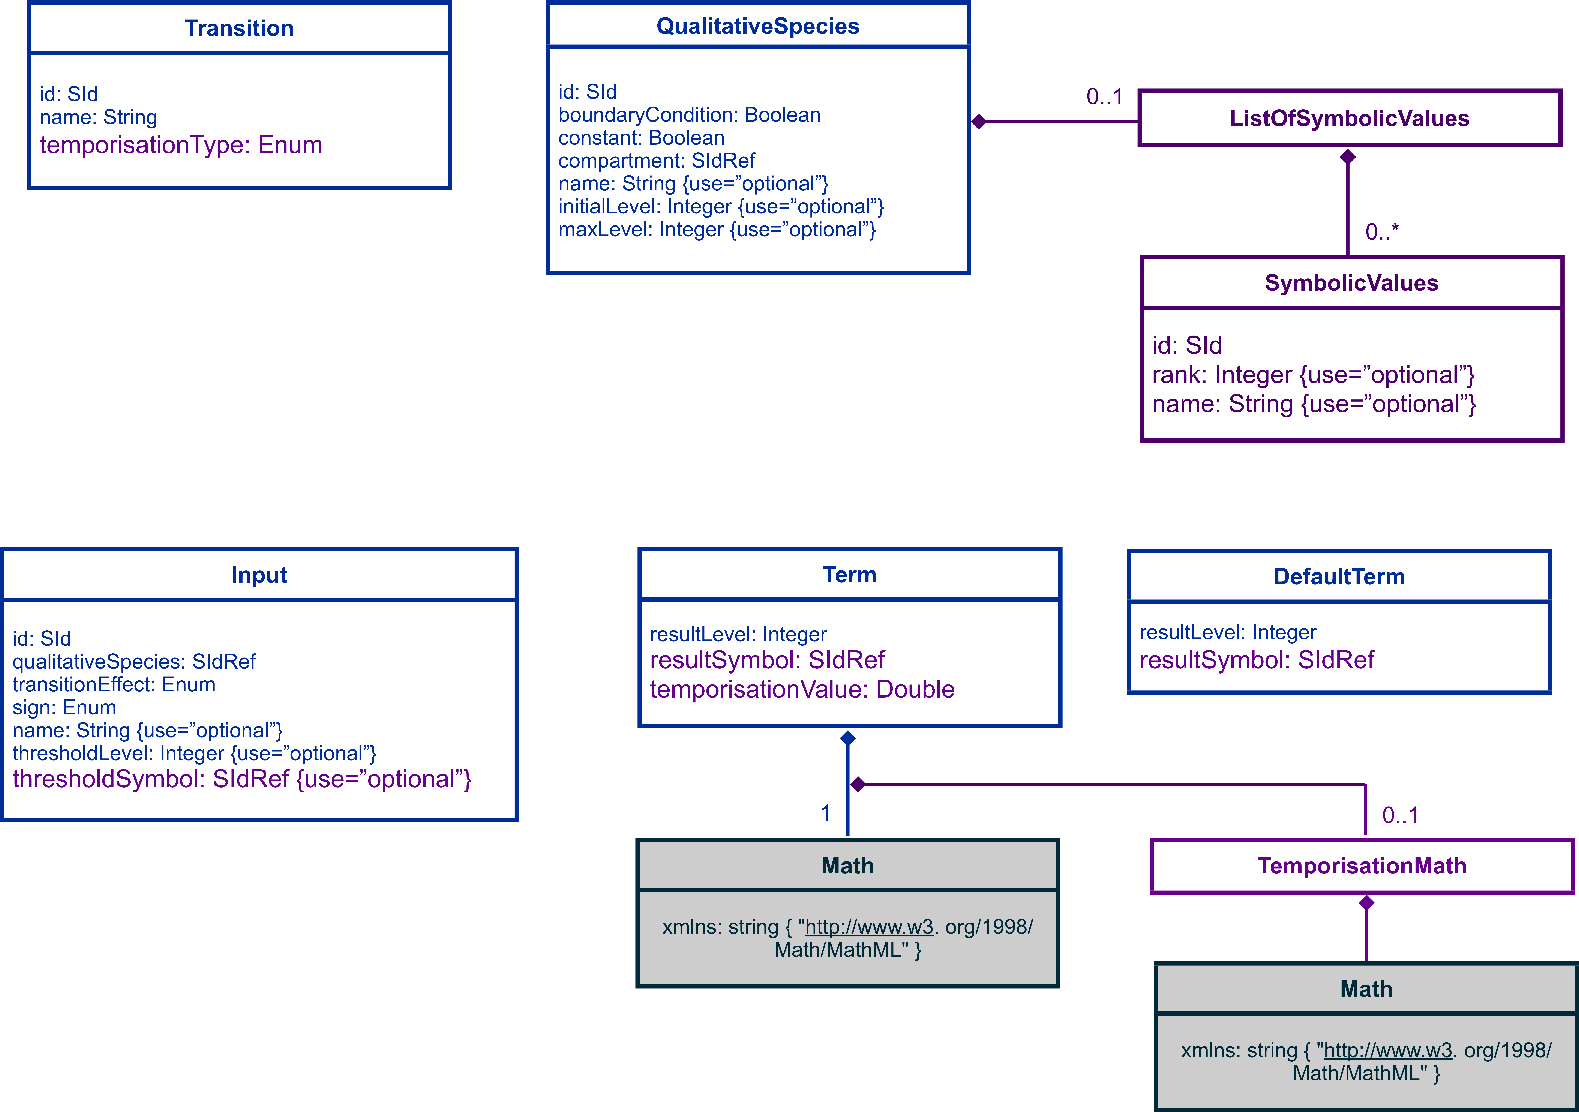
\includegraphics{figs/qual_future_directions.pdf}
%\caption {The definitions of the classe \listOf{SymbolicValues}, \qual{SymbolicValue} and \qual{TemporisationMath} and additional related attributes for existing classes.}
%  \label{qual_future_directions}
%\end{figure}


\subsection{Symbols}

\subsection*{Definition of \qualt{SymbolicValue}} % (fold)

\begin{figure}[hb]
  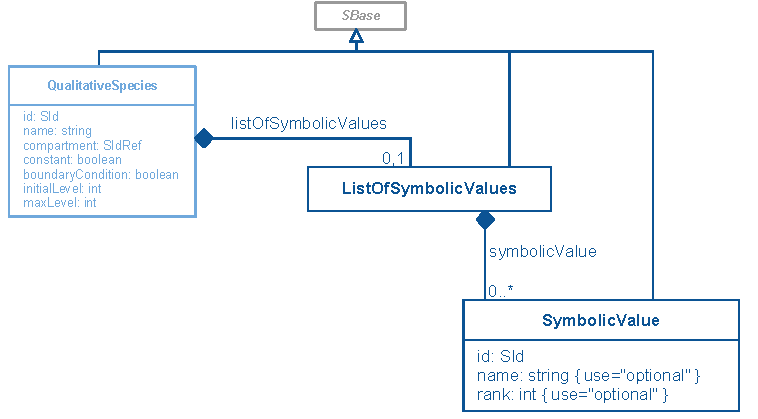
\includegraphics{figs/qual-qualitative-species-future-uml.pdf}
  \caption{Possible future extensions of the \QualitativeSpecies class.}
  \label{qual_future_directions}
\end{figure}

The \qual{QualitativeSpecies} element may contain at most one \listOf{SymbolicValues} that contains zero or more \qual{SymbolicValue}s. An empty list is allowed, and useful for e.g. adding annotations. 
The \qual{SymbolicValue} element defines a non instantiated parameter. Such symbols may represent the different solutions of piecewise linear differential equations, along with different thresholds.

\paragraph{The \attr{id} and \attr{name} attributes}
These attributes are used according to the SBML L3.1 Section 3.3. The attribute \attr{id} is mandatory and \attr{name} is optional. 

\paragraph{The \attr{rank} attribute}
The \attr{rank} is an \type{integer} that defines the position of the symbol in the \listOf{SymbolicValues}. This attribute is optional.


\paragraph{The \attr{thresholdLevel} and \attr{thresholdSymbol} attributes:} %% of Input
The \attr{thresholdLevel} is an \type{integer} and \attr{thresholdSymbol} is a \type{SIdRef}. They are optional and exclusive.

\paragraph{The \attr{resultLevel} and \attr{resultSymbol} attributes:} %% in FunctionTerm
The result of the term is described by a \attr{resultLevel} or a \attr{resultSymbol}. Both are optional, but one of them must be defined.


\const{assignmentSymbol}: The symbol associated to the \attr{qualitativeSpecies} is set to the \attr{resultSymbol} of the selected term.

\subsection{Temporisation}

\begin{figure}[hb]
  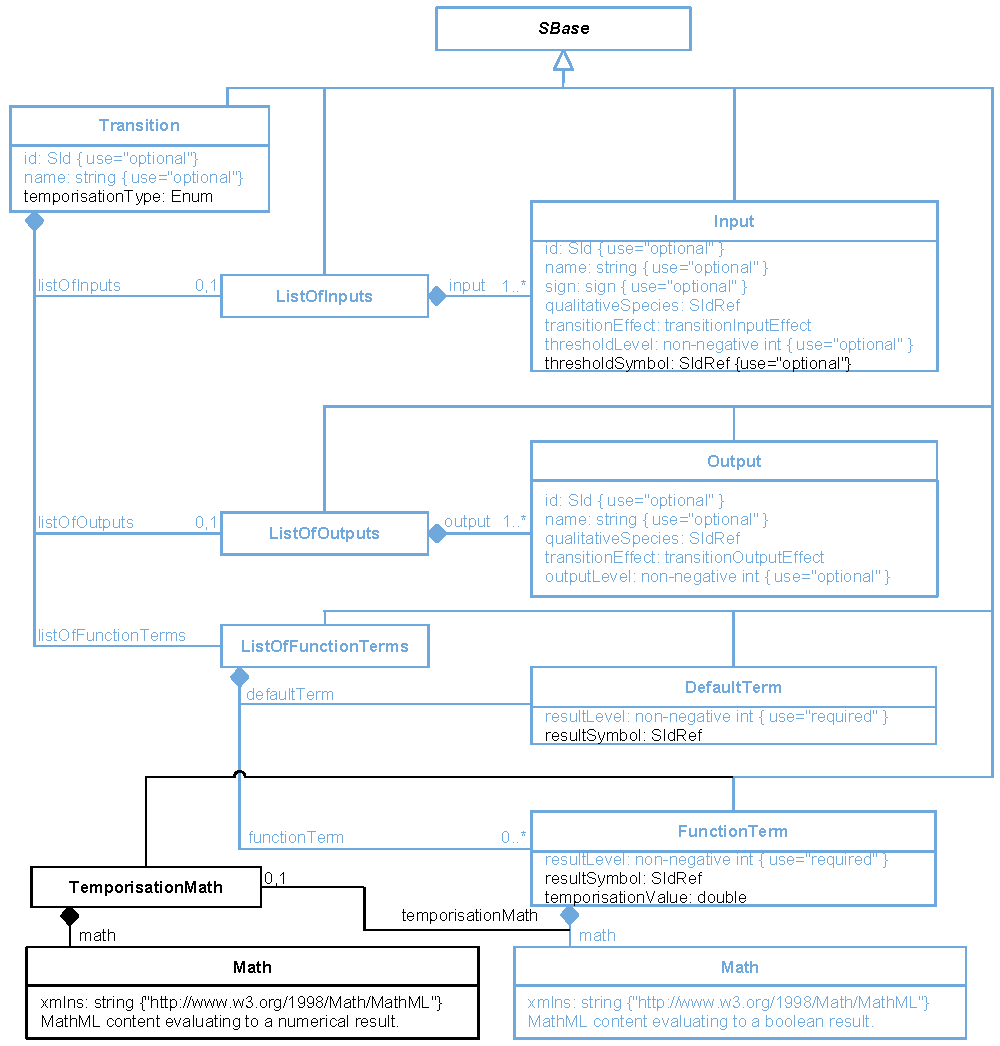
\includegraphics{figs/qual-transition-future-uml.pdf}
  \caption{Possible future extensions of the \Transition class.}
  \label{qual_future_directions}
\end{figure}

\paragraph{The \attr{temporisationType} attribute:} %% attribute of Transition
The \attr{temporisationType} is an \type{enumeration} the ``temporisation'' of the \qual{Transition}, that is the updating policy associated with the \qual{Transition}. It can be set to \const{timer}, \const{priority}, \const{sustain}, \const{proportion} or \const{rate}.
This attribute is optional. 



\paragraph{The \attr{temporisationValue} attribute and the \sbml{TemporisationMath} element:}
The attribute \attr{temporisationValue} and the element \sbml{TemporisationMath} allow the specification of the ``temporisation'' of the \qual{Transition} under the corresponding \qual{FunctionTerm}. Both are optional. Depending on the value of the \attr{temporisationType}, either one or both could be used.

The \attr{temporisationValue} is a \type{double}. The element \sbml{TemporisationMath} holds a MathML function returning a \type{double}. 

\hl{
\subsection{Classes of models and random models}}
\hl{
Several comments indicate that a future extension could support the representation of classes of models ({\it i.e.} models that are not fully parametrised, meaning that e.g. the logical rule of a component is incomplete), or random models, e.g. where several logical rules are associated to a component, the choice of a rule in the course of the dynamical evolution being arbitrary.
This might be done by revising the requirement of certain elements as well as the current semantics of {\em function terms}.}

\hl{\subsection{Interaction with SBML Core concepts}}
\hl{
At the time at which this Qualitative Modelling specification was developed, the policy and process for interacting with SBML Level 3 Core constructs was undefined. Thus, this particular specification does not facilitate the use of Core constructs. It is anticipated that in the future the specification will be extended to allow the use of these constructs; in particular Parameters and Events.
}

\subsection{Petri net models}

\textcolor{blue}{The current specification covers the needs of standard Petri Nets but provides a base for expansion to encompass more sophisticated modelling in this area. Both High Level Petri Nets (also referred to as Coloured PetriNets) and Timed PN should be achievable in future versions.}

\textcolor{blue}{We note that most PN models currently refer to metabolic or other reaction networks, and PN tools dedicated to this modelling framework often provides support for the SBML core format (see e.g. \cite{snoopy10}). }




\setcounter{secnumdepth}{-1}
% -*- TeX-master: "main"; fill-column: 72 -*-

\section{Acknowledgements}

We thank Andrew Finney, Nicolas Le Nov\`{e}re, Stefan Hoops, Martin Ginkel,
Wolfram Leibermeister, Ranjit Randhawa, Jonathan Webb, Frank Bergmann,
Sarah Keating, Sven Sahle, James Schaff, Chris Myers, and the sbml-comp
Package Working Group for prior work, suggestions, and comments that helped
shape the Hierarchical Model Composition package as you see it today.

We also thank with great enthusiasm the financial support of the National
Institutes of Health under grant R01 GM070923 to M. Hucka.


\clearpage
\bibliography{qual}


\end{document}
